\documentclass[english, 11pt]{article}
\usepackage{notes}
\usepackage{inconsolata}
\usepackage[shellescape]{gmp}
%\renewcommand{\sfdefault}{cmss}
%\renewcommand{\familydefault}{\sfdefault}
\newcommand{\thiscoursecode}{CS 246}
\newcommand{\thiscoursename}{Object-Oriented Software Development}
\newcommand{\thisprof}{Dr. Mark Prosser}
\newcommand{\me}{Liam Horne}
\newcommand{\thisterm}{Fall 2013}
\newcommand{\website}{LIHORNE.COM}
\usepackage{ifpdf}
\ifpdf
\DeclareGraphicsRule{*}{mps}{*}{}
\fi
% Headers
\chead{OOP}
\lhead{\thisterm}

%%%%% TITLE %%%%%
\newcommand{\notefront} {
\pagenumbering{roman}
\begin{center}

{\ttfamily \url{\website}} {\small}

\textbf{\Huge{\noun{\thiscoursecode}}}{\Huge \par}

{\Large{\noun{\thiscoursename}}}\\ \vspace{0.1in}

\vspace{0in}\includegraphics[scale=0.5]{logo.png}

  %\includegraphics[scale=0.1]{shield.png} \\
  {\noun \thisprof} \ $\bullet$ \ {\noun \thisterm} \ $\bullet$ \ {\noun {University of Waterloo}} \\

  \end{center}
  }
 \tikzstyle{class}=[
    rectangle,
    draw=black,
    text centered,
    anchor=north,
    text=black,
    text width=3cm,
    shading=axis,
    bottom color={rgb:red,222;green,222;blue,222},top color=white,shading angle=45]



%   ooooo      ooo   .oooooo.   ooooooooooooo oooooooooooo  .oooooo..o
%   `888b.     `8'  d8P'  `Y8b  8'   888   `8 `888'     `8 d8P'    `Y8
%    8 `88b.    8  888      888      888       888         Y88bo.
%    8   `88b.  8  888      888      888       888oooo8     `"Y8888o.
%    8     `88b.8  888      888      888       888    "         `"Y88b
%    8       `888  `88b    d88'      888       888       o oo     .d8P
%   o8o        `8   `Y8bood8P'      o888o     o888ooooood8 8""88888P'



\begin{document}
\renewcommand\familydefault{\sfdefault}
\sffamily
  % Notes front
  \notefront
  % Table of Contents and List of Figures
  \tocandfigures
  % Abstract
  \doabstract{These notes are intended as a resource for myself; past, present, or future students of this course, and anyone interested in the material. The goal is to provide an end-to-end resource that covers all material discussed in the course displayed in an organized manner. If you spot any errors or would like to contribute, please contact me directly. \\

  Brad Lushman: Any such notes have no official status in this course and we do not endorse their contents, nor will we point out or correct any errors in them.  Use at your own risk.}


  \section{Introduction}

  This course uses Linux. Thus one of the following are necessary
  \begin{itemize}
    \item a bash shell
    \item a Linux install
    \item Linux virtual machine
    \item ssh into linux.student.cs.uwaterloo.ca
    \item PuTTy, WinSCP, Cygwin, etc
  \end{itemize}

  This course is structured into understanding Linux shells (bash), using the C++ programming language, studying various tools and some software engineering concepts.

  \section{The Linux Shell}

  The Linux shell is an interface to the operating system. It provides a way to get the operating system to accept commands and carry out the necessary work, or to manage things for us. There are two kinds of interfaces; \textbf{graphical} and \textbf{command-line}.

  \begin{rem}
    A graphical shell is common on Windows and Mac. Operations typically include things like double-clicking, dragging, hovering, etc. In Linux, Gnome and KDE are examples. GUIs make simple tasks easy and intuitive. The shortshide however are that tasks can become harder to carry out as complexity increases.
  \end{rem}

  \begin{rem}
    Command line interfaces accept commands at a prompt and are traditional for UNIX/Linux. Windows has the "DOS" Command Prompt, and Mac is UNIX based. These interfaces have a steeper learning curve but are much more powerful than graphical interfaces. A typical command line interface would look something like this:
    \begin{lstlisting}[ numbers=none]
[mycomputer /var/nsm/] $
    \end{lstlisting}
  \end{rem}

  In this course we use \textbf{bash} (short for "Bourne Again Shell"). To check what shell you're using, run

  \begin{lstlisting}[numbers=none]
echo $0
  \end{lstlisting}

  \subsection{Linux File System}

  The file system consists of \textbf{files} (e.g., programs, data) and \textbf{directories}. Directories can contain other directories as well as files. Directories are arranged in hierarchical tree structure. The typical hierarchy is:

  \begin{center}
    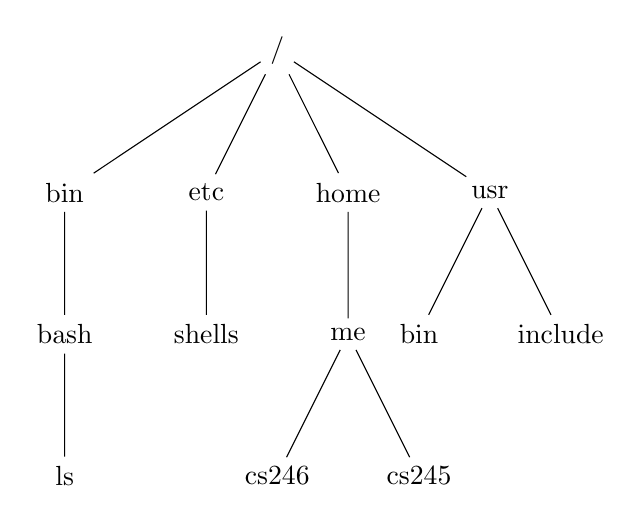
\begin{tikzpicture}[scale=1.2]
    \node[](z){\tc{/}}
      child{
        node[]{\tc{bin}}
          child{
          node[]{\tc{bash}}
          child{
          node[]{\tc{ls}}
          }
          }
      }
      child{
        node[]{\tc{etc}}
          child{
          node[]{\tc{shells}}
        }
      }
      child{
        node[]{\tc{home}}
        child{
          node[]{\tc{me}}
          child{
          node[]{\tc{cs246}}
          }
          child{
          node[]{\tc{cs245}}
          }
          }
      }
      child{
        node[]{\tc{usr}}
        child{
          node[]{\tc{bin}}
          }
          child{
          node[]{\tc{include}}
          }};
    \end{tikzpicture}
  \end{center}

  We can specify any file or directory by its \textbf{path} from the root. For example, {\ttfamily /var/nsm/bin/}.

  \begin{defn}[Current Directory]
    There is a notion of present working directory that, when in a bash shell, is the current directory that will provide an environment for commands to run in. Usually, a new bash shell will open to the home directory. The command {\ttfamily pwd} will return this directory. As well, each directory has a shortcut within itself, and is symbollicaly represented by "{\ttfamily .}".
  \end{defn}

  There are two kinds of paths.

  \begin{defn}[Relative Path]
    Relative path is a path that is referring to your current directory. For example, if {\ttfamily pwd} return {\ttfamily /home/} then any file I refer to or directory refers to what is in the {\ttfamily /home/} folder.
    \begin{lstlisting}[language=bash,numbers=none]
[var] $ pwd
/var
[var] $ cd mail/
[mail] $ pwd
/var/mail
    \end{lstlisting}
  \end{defn}

  \begin{defn}[Absolute Path]
    An absolute path starts with the root directory. For example {\ttfamily /home/} will always refer to exactly that directory, even if there is a {\ttfamily home} directory in some other directory.
  \end{defn}

  \begin{rem}
    The following special directories exist:
    \begin{itemize}
      \item {\ttfamily .} refers to the current directory. (relative)
      \item {\ttfamily ..} refers to the parent directory. (relative)
      \item {\ttfamily \textasciitilde} refers to the home directory. (absolute)
      \item {\ttfamily \textasciitilde userid} refers to the home directory of {\ttfamily userid}. (absolute)
    \end{itemize}
  \end{rem}

  \textbf{Change Directory} To change the current directory, use the \tc{cd} command. For example, \tc{cd /home/} takes you to the \tc{/home/} directory. \\
  \textbf{List Files/Directories} To list all files in the current directory, use the \tc{ls} command. For example, \tc{ls /home/} will list all files or directories in \tc{/home/}. To show hidden files, pass the \tc{-a} flag. \\
  \textbf{Create Directory} Use \tc{mkdir dirname} \\
  \textbf{Remove Directory} Use \tc{rmdir dirname} \\
  \textbf{Remove Directory AND Contents} \tc{rm -r dirname}

  \subsection{Wildcard Matching / Globbing}

  What if I want to see just the text files? (\tc{.txt} extension). The \tc{*} character symbolizes a "globbing" pattern, matching any string at all to it. Thus,
  \[ \mbox { \tc {ls *.txt }} \]
  will match all \tc{.txt} files and list them. The act of globbing by the command line is that the shell will substitute every file matching the expression and replaces the single term with multiple terms of matching files. If there is no match, the original glob considers the \tc{*} to be a literal character. For example,

  \[ \mbox{\tc{ls *.txt}} \iff \mbox{\tc{ls abc.txt def.txt ghi.txt}} \]

  This is a bash constant, and therefore works for every command.

  \subsection{Variables}

  Declaration of a variable is done like so: \tc{x=1} (no spaces!) and accessing variables in other contexts uses a dollar sign, so \tc{echo \${x}} will return 1. For example
  \begin{lstlisting}[language=bash,numbers=none]
    $ dir=~/cs246
    $ echo ${dir}
    /home/rmprosse/cs246
    $ ls ${dir}
    a0 a1 a2 etc
  \end{lstlisting}

  Note that the \tc{$\sim$} is expanded before the variable is assigned. \\

  In bash there are several "global" variables that are already set up for you. To list these variables, use the \tc{env} command. For example,
  \begin{lstlisting}[language=bash,numbers=none]
$ env
SHELL=/bin/bash
USER=lihorne
PATH=/usr/local/Cellar/emacs/24.3/bin:/usr/local/bin:/bin:/usr/sbin:/sbin:/usr/bin:/usr/texbin
PWD=/Users/lihorne
LANG=en_CA.UTF-8
HOME=/Users/lihorne
LOGNAME=lihorne
_=/usr/bin/env
  \end{lstlisting}

  The most important of these global variables is the \tc{PATH}. The path is a colon (":") delimited list of directories that are searched in order when a command is issued.

  \subsection{Quoting}

  Quotes are used to control how the shell interprets strings. Note that globbing does not occur inside quoted strings, they are treated as literals. As well, single quotes protect everything except a single quote, and double quotes protect everything except double quotes (\tc{"}), back quotes (\tc{`}), and dollar signs (\tc{\$}). When inside double quotes, these characters have to be escaped. Escaping is done using the backslash (\tc{\symbol{92}}).

  \begin{exmp}
  \
  \begin{lstlisting}[language=bash,numbers=none]
$ echo $PATH
/usr/local/bin:/bin:/usr/sbin:/sbin:/usr/bin:/usr/texbin
$ echo "$PATH"
/usr/local/bin:/bin:/usr/sbin:/sbin:/usr/bin:/usr/texbin
$ echo '$PATH'
$PATH
  \end{lstlisting}
  \end{exmp}

  What if I wanted to use the strijng \tc{"*.txt"} including the quotes? Simply put it all inside single quotes, or double quotes with escaping like this
  \begin{lstlisting}[language=bash,numbers=none]]
$ echo '"*.txt"'
"*.txt"
$ x="\"*.txt\""
$ echo ${x}
"*.txt"
  \end{lstlisting}

  \subsection{Input/Output Redirection}
  There is a command called \tc{cat} that displays the contents of a file or returns input. So, \tc{cat hello.txt} returns \tc{hello, world}. If there is no argument \tc{cat} waits for input and returns that input after it had completed. Hit \tc{\^{}C} to stop the process, and \tc{\^{}D} to stop the input. If however we wanted to redirect the output of \tc{cat} then we can use a redirection operator like so:
  \begin{lstlisting}[language=bash,numbers=none]
$ cat hello.txt
hello, world
$ cat > hello.txt
my name is liam
^D
$ cat hello.txt
my name is liam
  \end{lstlisting}

In general, \tc{command args > file} will redirect the output from \tc{command args} to \tc{file}. This is called \textbf{output redirection}. We can do both input and output redirection using redirection, for example \tc{cat < inputfile.txt > outputfile.txt} will take the contents of \tc{inputfile.txt} and overwrite \tc{outputfile.txt} with it. \\
Note that every process has 3 streams. They are
\begin{enumerate}
  \item Standard Input - which is input into a program
  \item Standard Output - that a program outputs
  \item Standard Error - that a program outputs, it is a seperate output stream for error messages and is seperate from regular output
\end{enumerate}
By default, \tc{stdin} is conected to the keyboard, \tc{stdout} and \tc{stderr} are connected to the screen. Input redirection connects \tc{stdin} to a file and output redirection connects \tc{stdout} to a file. We can redirect \tc{stderr} as well, for example \tc{program < in.txt > out.txt 2> errlog.txt}. The \tc{2>} will only output errors to the file. Note that redirection will create the file if necessary and \textbf{replace entire contents}. Additionally, you can use \tc{$>>$} to \textbf{append} output.

\subsection{Pipes}

  Pipes let you connect the output of one program to the input of another (just like a pipe, wow). Connecting two commands is done using a vertical bar ("|"). This sets the second program's \tc{stdin} to the first program's \tc{stdout}.

  \begin{exmp}
    How many words occur in the first 20 lines of \tc{myfile.txt}?
    We can use this series of commands
    \begin{lstlisting}[language=bash,numbers=none]
$ head -20 myfile.txt | wc -w
42
    \end{lstlisting}
  \end{exmp}

  This example illustrates using the output of \tc{head -20 myfile.txt} which is the first 20 lines of a file, and using it as the input for \tc{wc -w} which counts the number of words in the input.

  \begin{exmp}
    Suppose \tc{words.txt}, \tc{words2.txt}, $\ldots$ contains lists of words, one word per line. Print a duplicate-free list of all the words in these files, \tc{words*.txt}. We will consider two programs that are useful in this problem.
    \begin{itemize}
      \item[i.] \tc{uniq} - removes adjacent duplicate lines
      \item[ii.] \tc{sort} - sorts lines
    \end{itemize}
    Therefore if the input is sorted, uniq removes all duplicates. Our solution is the command
    \begin{center}
      \tc{cat words*.txt | sort | uniq}
    \end{center}
  \end{exmp}

  \subsection{Command Substitution}

  Can we use the output of a command as a \textbf{parameter} of another? The answer is yes, we simply put the command in \textbf{backquotes} (or quasiquotes). For example, \tc{echo `date`}
   will execute the \tc{date} command and use it as input into \tc{echo}.

   \begin{rem}
     Recall that double quotes do not protect back quotes, shell expands back quotes inside double quotes. For example \tc{echo \" `date` \"} has the same meaning. Alternatively, we can use \tc{\$()} instead of \tc{` `}. For example, \tc{echo \$(date)} has the same effect.
   \end{rem}

   \subsection{Grep - pattern matching in text files}

   We now study a new tool called \tc{grep}, which stands for "Global Regular Expression Print". There is also an extended version called \tc{egrep} which is equivalent to \tc{grep -E}, which interprets a pattern as an extended regular expression (i.e. forces grep to behave as egrep). The general format is
   \begin{center}
     \tc{grep pattern file}, which prints lines in \tc{file} which match \tc{pattern}.
   \end{center}
   \begin{exmp}
     Suppose we want to print all lines in our websites homepage, \tc{index.html} that contain the pattern \tc{cs246}. We simply call \tc{grep cs246 index.html}.
   \end{exmp}
   How many lines match?
   \begin{center}
     \tc{grep cs246 index.html | wc -l} \ or \ \tc{grep -c cs246 index.html}
   \end{center}
   We can use expressions called \textbf{regular expressions}; note that this is a completely seperate idea to globbing, and although there are many things in common and the syntax is similar, they are different.
   \begin{exmp}
     Search for \tc{cs246} or \tc{CS246}. The solution involes a regex that checks on the first alphabetic letters.
     \begin{center}
       \tc{grep -E "cs246|CS246" index.html} \ or \ \tc{grep -E "(cs|CS)246" index.html}
     \end{center}
     Observe that the parentheses allow grouping for the "or" operator "|". Some more identical commands include \tc{egrep "(c|C)(s|S)246" index.html} (which included mismatches of upper or lowercase characters) or \tc{egrep "[cC][sS]246" index.html}.
   \end{exmp}

   \begin{notation} \
     \begin{itemize}
       \item \tc{[$a_1a_2a_3\ldots a_n$]} will match any character \tc{$a_i$} in between \tc{[} and \tc{]}. So, \tc{[abc] $\equiv$ a|b|c}.
       \item \tc{[\^{}$a_1\ldots a_n$]} will match anything \textbf{except} the characters mentioned.
       \item To denote an optional preceding character, use the \tc{?} character. For example \tc{cs ?246} will match both \tc{cs246} and \tc{cs 246}.
       \item To denote optional preceding characters repeated 0 or more times, use \tc{*}. For example, \tc{cs*246} will match \tc{cs246} and \tc{cssssssssss246} and \tc{c246}.
       \item To denote a single instance of any character, use \tc{.} (for example, \tc{.*} denotes 0 or more of any character, which mimics globbing)
       \item The caret \tc{\^{}} has a different meaning at the beginning of a line. In the case
       \begin{center}
         \tc{egrep "\^{}cs246" index.html}
       \end{center}
       indicates lines starting with \tc{cs246}.
       \item Similarly, the dollar sign \tc{\$} indicates the end of a line. So,
       \begin{center}
         \tc{egrep"\^{}cs246\$" index.html}
       \end{center}
       will match lines containg \textbf{only} \tc{cs246} and nothing else.
       \item The \tc{+} sign will match 1 or more of the preceding pattern
     \end{itemize}
   \end{notation}
   \begin{exmp}
     Print all lines of even length.
     \begin{center}
       \tc{egrep "\^{}(..)*\$" index.html}
     \end{center}
   \end{exmp}
   \begin{exmp}
     Print all files in current directory whose names contain \textbf{exactly one a}.
     \begin{center}
       \tc{ ls | grep -E "\^{}[\^{}a]*a[\^{}a]*\$" }
     \end{center}
   \end{exmp}

   \subsection{Permissions}

   Recall the \tc{ls -l} will print the \textbf{long form} directory listing. For example
   \begin{lstlisting}[language=bash,numbers=none]
$ ls -l
total 0
drwxr-xr-x+  4 lihorne  staff   136 16 Sep 20:57 Desktop
drwxr-xr-x+ 10 lihorne  staff   340 14 Sep 10:35 Documents
drwxr-xr-x+ 12 lihorne  staff   408 17 Sep 11:32 Downloads
drwx------\@  9 lihorne  staff   306 15 Sep 16:37 Dropbox
drwx------\@ 60 lihorne  staff  2040 14 Sep 02:06 Library
drwxr-xr-x+  6 lihorne  staff   204 14 Sep 04:55 Movies
drwxr-xr-x+  6 lihorne  staff   204 14 Sep 04:55 Music
drwxr-xr-x+  9 lihorne  staff   306 14 Sep 04:55 Pictures
drwxr-xr-x+  6 lihorne  staff   204 21 Aug 19:28 Public
   \end{lstlisting}

   These listings mean,
   \begin{center}
     \tc{\ubt{d}{type}\ubt{rwxr-xr-x+}{permissions} \ubt{6}{\#links} \ubt{lihorne}{owner}  \ubt{staff}{group}   \ubt{204}{size} \ubt{21 Aug 19:28}{last modified} \ubt{Public}{name}}
   \end{center}

   We're interested in the permissions. The permissions are split into three pieces,
   \begin{center}
     \tc{\ubt{rwx}{user}\ubt{r-x}{group}\ubt{r--}{other}}
   \end{center}
   \begin{itemize}
     \item \textbf{user bits:} what the file's owner can do with it
     \item \textbf{group bits:} what members of the file's group can do with it (other than owner)
     \item \textbf{other bits:} what other users can do
   \end{itemize}
   Each set has
    \begin{center}
    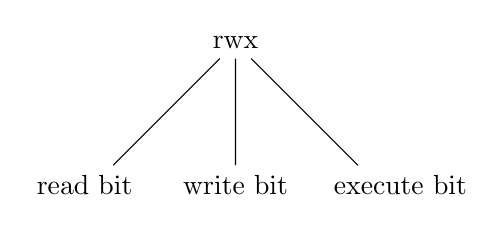
\begin{tikzpicture}[scale=1.2]
    \node[](z){\tc{rwx}}
      child{
        node[]{\tc{read bit\ \ \ }}
          }
          child{
          node[]{\tc{write bit}}
          }
          child{
          node[]{\tc{\ \ \ \ \ execute bit}}
      };

    \end{tikzpicture}
  \end{center}
  What these mean depends on the type of file. \\

  \begin{tabular}{l | l | l}
    Bit & Ordinary File & Directory \\
    \hline
    r & file can be read & contents can be read (i.e., \tc{ls}) \\
    w & file can be modified & contents can be modified (i.e., add / remove) \\
    x & files can be executed & directory can be navigated (i.e., in \tc{cd})
  \end{tabular}

  \begin{note}
    If a directory's \tc{x} bit is not set, it is not accessible whatsoever; no file or subdirectory within it is reachable.
  \end{note}

  \begin{rem}
    We list some more features of \tc{grep}:
    \begin{itemize}
      \item \tc{grep -v} is an inverted grep, it displays the lines that \textbf{don't} match.
      \item \tc{ls} \textbf{pipes} output as a column (not line) (detects if \tc{stdout} is a terminal).
      \item \tc{pcrgrep} is a \tc{grep} variant with a multiline option (\tc{-m}).
      \item Use a dash within \tc{[]} to specify range. For example, \tc{[0-9],[a-z]} are ranges over the first 10 digits and the 26 lowercase letters.
    \end{itemize}
  \end{rem}

  We can use the command \tc{chmod} which stands for "change permissions" to alter some of these bits. The general format is
  \begin{center}
    \tc{chmod mode file}
  \end{center}
  The term \tc{mode} is formatted such that there are three ownership groups, \\
  \begin{center}
  \begin{tabular}{l | l | l}
    Ownership Class & Operator & Permissions \\
    \hline
     \tc{u} for user (owner) & \tc{+} to add permission & \tc{r} for read \\
     \tc{g} for group & \tc{-} to remove permission & \tc{w} for write \\
     \tc{o} for other & \tc{=} to set permission exactly & \tc{x} to execute \\
     \tc{a} for all (u,g, and o)
  \end{tabular}
  \end{center}

  \subsection{Shell Scripts}

  A shell script is a file containing a sequence of shell commands and is executed as a program.

  \begin{exmp} \
    \begin{lstlisting}[language=bash]
#!/bin/bash      # <-"she-bang"
date             # (tells Linux to execute
whoami           #  this file as a bash script)
pwd
    \end{lstlisting}
    We first give the file execute permissions using
    \begin{center}
        \tc{chmod u+x myscript}
     \end{center}
     Then run the file with \tc{./myscript}.
  \end{exmp}

  \begin{note}
    Command-line arguments are accessed as \textbf{variables} such as \tc{\$\{1\}, \$\{2\},} etc
  \end{note}

  \begin{exmp}
    Check whether a word is in the dictionary. We create a file \tc{isItAWord} that contains the following:
    \begin{lstlisting}[language=bash]
#!/bin/bash
egrep "^$1$" /usr/share/dict/word
    \end{lstlisting}
    The script checks a dictionary file for the regex that is a line of only the word given as an argument to the script. Thus,
    \begin{center}
      \tc{./isItAWord hello}  \ \ \ \ prints \tc{hello} if it is there, nothing otherwise.
    \end{center}
  \end{exmp}

  \begin{exmp}
    A "good" password is not in the dictionary. Determine whether a word might be a "good" password.
    \begin{lstlisting}[language=bash]
#!/bin/bash
egrep "^$1$" /usr/share/dict/words > /dev/null
    \end{lstlisting}
    where \tc{/dev/null} is a directory that suppresses output.
  \end{exmp}

  \begin{note}
    Every program returns a status code when finished. For example, \tc{grep} returns 0 if a match was found and 1 otherwise. In Linux, 0 means success and nonzero means a failure. Essentially,
    \[ \mbox{\tc{program}} = \piecewise{\mbox{\tc{success}}}{if status code is 0}{\mbox{\tc{failure}}}{otherwise} \]
  \end{note}

  The variable \tc{\$\{?\}} is the status code of the most recently executed program. So, we now add the following to our script:
  \begin{lstlisting}[language=bash]
if [ ${?} -eq 0 ]; then
  echo Not a good password
else
  echo Maybe a good password
fi
  \end{lstlisting}

  \begin{note} We have a particular usage for this program that we want, and that is that the user should pass exactly one argument. To ensure this use, or rather to provide helpful error messages should it be used incorrectly, we use another special variable, \tc{\$\#}.
    \end{note}

    It's common to write a function with usage information as shown here:
    \begin{lstlisting}[language=bash]
usage () {
  echo "Usage: $0 password" >&2
  exit 1
}

if [ ${#} -ne 1 ]; then
  usage
fi
    \end{lstlisting}

    And the complete script then defines a usage function, checks the number of arguments, runs the dictionary lookup, and finally returns whether or not a password is deemed to be good.
    \begin{lstlisting}[language=bash]
#!/bin/bash
# Answers whether a candidate word might be a good password

usage () {
  echo "Usage: $0 password" >&2
  exit 1
}

if [ ${#} -ne 1 ]; then
  usage
fi
egrep "^$1$" /usr/share/dict/words > /dev/null

if [ $? -eq 0 ]; then
  echo Not a good password
else
  echo Maybe a good password
fi
    \end{lstlisting}

\begin{notation}
  The general format for if statements is
  \begin{lstlisting}[language=bash]
if [ condition ]; then
  ...
elif [ condition ]; then
  ...
else
  ...
fi
    \end{lstlisting}
\end{notation}
    \begin{exmp}
      We'll have a look at an example of loops. This example prints the number 1 to \tc{\$1}. This file is from \tc{lectures/shell/scripts/count}.
  \begin{lstlisting}[language=bash]
#!/bin/bash
# count limit ---counts the numbers from 1 to limit

usage () {
  echo "Usage:  $0 limit" 1>&2
  echo "  where limit is at least 1" 1>&2
  exit 1
}

if [ $# -ne 1 ]; then
  usage
fi

if [ $1 -lt 1 ]; then
  usage
fi

x=1
while [ $x -le $1 ]; do
  echo $x
  x=$((x + 1))
done
    \end{lstlisting}
    \begin{note} \
      \begin{itemize}
        \item \tc{1>\&2} "ties" \tc{stdout} (1) to \tc{stderr} (2)
        \item \tc{\$(( ... ))} does \textbf{arithmetic expansion}
      \end{itemize}
    \end{note}
    \end{exmp}

    Now suppose we want to loop over a list, this next example portrays this.

    \begin{exmp}
      Rename all \tc{.C} files to \tc{.cc}. This next script is from \tc{lectures/shell/scripts/renameC}.
      \begin{lstlisting}[language=bash]
#!/bin/bash
# Renames all .C files to .cc

for name in *.C; do
  mv ${name} ${name%C}cc
done
      \end{lstlisting}
      \begin{note} \
      \begin{center}
\tc{for v in list} : sets variable v to each word in list \\
\tc{\$\{name\%C\}} : returns the value of the name variable without the trailing C
      \end{center}
      \end{note}
    \end{exmp}

    \begin{exmp}
      Write a script that returns the date of the last friday of this month. \\ To accomplish this we use the \tc{awk} command in conjunction with the \tc{cal} command. Thus one possible command to accomplish this is. For example,
      \begin{center}
        \tc{cal January 2014| awk '{print \$6}' | grep [0-9] | tail -1}
      \end{center}
      The following script is from \tc{/shell/scripts/payday}. There are two steps, the first is to find the date and the second is to report the answer.
      \begin{lstlisting}[language=bash]
#!/bin/bash
# Returns the date of the next payday (last Friday of the month)
# Examples:
# payday (no arguments) -- gives this month's payday
# payday October 2012 -- gives payday in October 2012

answer () {
  if [ $2 ]; then
     preamble=${2}
  else
     preamble="This month"
  fi
  if [ $1 -eq 31 ]; then
    echo "${preamble}'s payday is on the ${1}st."
  else
    echo "${preamble}'s payday is on the ${1}th."
  fi
}

answer `cal $1 $2 | awk '{print $6}' | grep "[0-9]" | tail -1` $1
      \end{lstlisting}
    \end{exmp}

    \begin{exmp}
      The following string counts the number of lines that a word appears in a file.
      \begin{lstlisting}[language=bash]
#!/bin/bash
# countWords word file
#  Prints the number of times word occurs in file

x=0
for word in `cat "$2"`; do
  if [ $word == $1 ]; then
    x=$((x + 1))
  fi
done
echo $x
      \end{lstlisting}
    \end{exmp}

    \subsection{Testing}

    Testing is the essential part of software engineering; it often takes much more time than expected. Additionally, it is ongoing, not just at the end, and tests should be written before the program is written. Test suites are used for streamlining the process of testing. Note that testing is not debugging, and testing must happen first. \\ Testing can't guarantee your program is correct, it can only prove it is incorrect. Ideally, the developer and tester are different people (but not in this course).

    \begin{itemize}
      \item Human testing - people examine code, looking for flaws. This includes code inspection, and walkthroughs.
      \item Machine testing - systematically run programs through test input, check the output against specifications. Can't test everything, so choose cases carefully.
    \end{itemize}

    There are two main approaches to testing.

    \begin{itemize}
      \item \textbf{Black-box Testing} - no knowledge of implementations
      \item \textbf{White-box Testing} - full knowledge of implementation
    \end{itemize}

    Gray-box testing could be considered testing done with some knowledge of implementation but not all. \\
    Typically, black-box testing is the first to occur and is then supplemented by white-box testing. We analyze some techniques of both types. \\

    \textbf{Black-Box}
    \begin{itemize}
      \item Think about classes of inputs to avoid redundancy. For example, numeric ranges, positive, negative, etc.
      \item Boundary cases (edge cases), consider boundaries between classes
      \item Intuition and experience should be used to guess errors
      \item Extreme cases, push the limits of the program
    \end{itemize}

    \textbf{White-Box}
    \begin{itemize}
      \item Check all logical paths
      \item Test to make every function run
    \end{itemize}

    \textbf{Strategies}
    \begin{itemize}
    \item Single Component:
      \begin{itemize}
        \item Unit testing: test individual components (e.g., small code, program, class)
      \end{itemize}
    \item Multiple Component:
       \begin{itemize}
         \item Integration testing: test interaction between multiple components
       \end{itemize}
    \item All Components:
    \begin{itemize}
      \item Functional testing: program works as expected in normal conditions
      \item Regression testing: test modified version of a previously validated program.
      \item System testing: test the functionality, performance, reliability, and security of the entire system
      \item Performance testing: program efficiency
      \item Volume testing: ability to handle inputs in different volumes (small and large)
       \item Stress testing: ability to handle extreme volume of data in limited amount of time
       \item Acceptance testing: Operating the system in the user environment with standard user input scenario
    \end{itemize}
    \end{itemize}

    \section{C++}

    \subsection{Introduction - Hello World}

    In C, the Hello World program looks like this:
    \begin{lstlisting}[language=c]
#include <stdio.h>
int main() {
  printf("Hello World\n");
  return 0;
}
    \end{lstlisting}
    The C++ version looks like this:
\begin{lstlisting}
#include <iostream>
using namespace std;
int main() {
  cout << "Hello World" << endl;
  return 0;
}
\end{lstlisting}
\begin{note}
  In C++, the \tc{main} program must return an \tc{int} (status code). Emitting the return statement will however return 0 anyway. Note that \tc{stdio.h} and \tc{printf} are still available in C++, but the preferred method is as shown above. That is, using the header \tc{<iostream>}, and with output mechanism \tc{std::cout << ... << ... << std::endl} (meaning there can be multiple uses of the \tc{<<} operator). \\
  \tc{std::cout} is the standard output stream, and \tc{std::endl} is the end of line indicator. \\
  \tc{using namespace std;} lets you refer to \tc{std::cout} and \tc{std::endl} without the \tc{std::}. \\

  Most C programs are valid C++ programs, that is C++ is a near-perfect superset of C.
\end{note}

To compile a C++ program: \tc{g++ program.cc} \ubt{\tc{-o program}}{specifies name of executable}. If the name is emitted, then the compiled program is called \tc{a.out}. Then executing is as simple as running \tc{./program}.

\subsection{C++ Input \& Output}

There are 3 I/O Stream objects:
\begin{itemize}
  \item \tc{cin} - reading from \tc{stdin}.
  \item \tc{cout} - printing to \tc{stdout}.
  \item \tc{cerr} - printing to \tc{stderr}.
\end{itemize}
The I/O operators are:
\begin{itemize}
  \item \tc{<<} - "put to" (output).
  \item \tc{>>} - "get from" (reading).
\end{itemize}
\begin{exmp}
  \item \tc{cin >> x} means getting data from \tc{cin} and writing it to \tc{x}.
  \item \tc{cout << x} means taking \tc{x} and writing it to \tc{stdout}.
  \item \tc{cerr << x} means writing \tc{x} to \tc{stderr}.
\end{exmp}

\begin{note}
  \tc{cin >>} ignores whitespace (tabs, spaces, newlines). That is, \tc{cin >> x >> y;} looks for two integers seperated by whitespace.
\end{note}

Some scenarios:
\begin{itemize}
  \item[(1)] What if the input doesn't contain an integer next? Then the statement fails, and the variable is not assigned.
  \item[(2)] What happens if input is exhausted before we get two integers? Then the statement fails, and the variable is not assigned.
\end{itemize}

How do we detect if either of these scenarios has occurred? Then,
\begin{center}
  read failed $\implies$ \tc{cin.fail()} returns \tc{true}. \\
  end-of-file reached $\implies$ \tc{cin.eof()} \textbf{and} \tc{cin.fail()} will return true, but not until the attempted read fails.
\end{center}

\begin{exmp}
  Read integers from \tc{stdin}, then echo them one per line to \tc{stdout}. Stop when the end of the file is reached or the read fails. \\
  Version 1:
  \begin{lstlisting}
#include <iostream>
using namespace std;
int main() {
  int i;
  while (true) {
    cin >> i;
    if (cin.fail()) break;
    cout << i << endl;
  }
}
\end{lstlisting}
\end{exmp}

\begin{note}
  \tc{cin} can be used as a condition in an if statement, since
  \begin{center}
    \tc{if (cin)} $\iff$ if (\tc{!cin.fail()})
  \end{center}
\end{note}
  How does this work? The if statement can use booleans, integers, or pointers as conditions. The compiler changed \tc{cin} to either 0 or the address of \tc{cin}. This is because \tc{cin} is a pointer, a reference to an object.

  Note that \tc{>>} is a function under \tc{cin}. That is,
  \begin{itemize}
    \item \tc{cin >> x} is equivalent to \tc{cin.>>(x)}
    \item \tc{>>} returns \tc{cin} itself
    \item This allows: \tc{cin >> x >> y} (which can be written as \tc{cin.>>(x).>>(y);}, which is then \tc{cin.>>(y)})
  \end{itemize}

  Also note that \tc{cin} is of type \tc{istream}.

  \begin{exmp}
  This example reads all integers from \tc{stdin} and echos them, one per line, to \tc{stdout}. It skips non-integer inputs. Note that \tc{cin.clear()} clears the internal error state and \tc{cin.ignore()} removes the part in input stream that generated the error.
    \begin{lstlisting}
#include <iostream>
using namespace std;

int main () {
  int i;
  while (true) {
    if (!(cin >> i)) {
      if (cin,eof()) break;
      else {
        cin.clear();
        cin.ignore();
      }
    }
    else {
      cout << i << endl;
    }
  }
}
    \end{lstlisting}
  \end{exmp}

  \subsection{Strings}

  C-like strings, that is null-terminated character arrays (\tc{char[], char*}), are well supported in C++. That is a string "Hello" can be defined like \tc{char mystr[] = "Hello";} where it is represented like [H][e][l][l][o][null]. C++ has a \tc{std::string} class that can be used like a basic data type. This reduces the maintenance overhead (e.g., memory management) and is more reliable (it hides the null character). Additionally, they can grow and shrink as needed, and are safer to manipulate. \\

  We can use the following \tc{string} operators
  \begin{itemize}
    \item == Equality
    \item != Inequality
    \item <,>,<=,>= Comparison
    \item s.length Length
    \item s[i] Character extraction
    \item s = s1 + s2 Concatenate (or +=)
  \end{itemize}

  This requires adding
  \begin{lstlisting}
#include <string>
using namespace std;
  \end{lstlisting}
Creating and initializing a string is done like this:
\begin{lstlisting}
string s1;                        // initialize to empty
string s2("My string in C++");    // initialize by constructor
string s3 = "my value";           // initialize by assignment
string s4 (s2);                   // initialize by another string
s2 = "another string";            // directly assign value, no strcpy
s2 = s1;
\end{lstlisting}
Strings can also be concatenated using the \tc{+} operator:
\begin{lstlisting}
string s1 = "Hello";
string s2(" world");
string s3 = s1 + " " + s2 + "!";
cout << s3 << endl;
cout << (s1 + " my" + s2 + ".") << endl;
\end{lstlisting}

However, strings can still be accessed as though they are characters in an array. So,
\begin{lstlisting}
string city = "Waterloo";
for (int i = 0; i < city.length(); i++) {
  cout << city[i] << " - ";
}
\end{lstlisting}
would return \tc{W - a - t - e - r - l - o - o -}. \\

\tc{cin} reads strings with the following semantics:
\begin{itemize}
  \item discard leading spaces
  \item read non-white characters into string
  \item stop at next whitespace character
\end{itemize}
To read the entire line, including the leading spaces, use \tc{getline(cin, str);}. \\

Refer to \url{http://www.cplusplus.com/reference/string/string/} for some useful \textbf{methods} from the string class.

\subsection{I/O Manipulation}

The behaviour of \tc{cout} can be controlled using I/O manipulations. The following header must be included:
\begin{lstlisting}[numbers=none]
#include <iomanip>
\end{lstlisting}
Maniuplators are not variables for input / output but rather control the I/O formatting for all literals / variables after it, continuing to the next I/O expression for a specific stream file. Except for \tc{setw}, they all apply to all proceeding values. \\
\begin{center}
\begin{tabular}{l | l}
\tc{oct} & integral values in octal \\
\tc{dec} & integral values in decimal \\
\tc{hex} & integral values in hexadecimal \\
\tc{left} / \tc{right} (default) & values with padding after / before values \\
\tc{boolalpha} / \tc{noboolalpha} (default) & bool values as false / true instead of 0/1 \\
\tc{showbase} / \tc{noshowbase} (default) & values with / without prefix 0 for octal and 0x for hex \\
\tc{showpoint} / \tc{noshowpoint} (default) & print decimal if no fraction \\
\tc{fixed} (default) / scientific & float-point values without / with exponent \\
\tc{setprecision(N)} & fraction of float-point values in maximum of $N$ columns \\
\tc{setfill(`ch`)} & padding character before / after value (default blank) \\
\tc{setw(N)} & next value only in minimum of $N$ columns \\
\tc{endl} & flush output buffer and start new line (output only) \\
\tc{skipws} (default) / \tc{noskipws} & skip whitespace characters (input only)
\end{tabular}
\end{center}

\begin{note} Manipulators and Floats
\begin{itemize}
  \item fixed - fixed decimal place (no exponent)
  \item scientific - scientific notation (use exponent)
\end{itemize}
The default is neither fixed not precision, precision meand number of significant digits to display after (not including) decimal point.
\end{note}

\begin{exmp}
To produce formatted output showing decimal, octal, and hexadecimal values for 16 through 20:
\begin{lstlisting}
cout << showbase
     << setw(6) << "Dec"
     << setw(6) << "Oct"
     << setw(6) << "Hex" << endl;
for (int i = 16; i < 20; ++i) {
  cout << dec << setw(6) << i
       << oct << setw(6) << i
       << hex << setw(6) << i << endl;
}
\end{lstlisting}
\end{exmp}

\subsection{Working with files}

In C we use \tc{fopen}, then \tc{fscanf}, then finally \tc{fclose}. Note that \tc{fscanf} returns the number of arguments read, and -1 on error. \tc{fscanf} does not take care of string overflow. The C example:

\begin{lstlisting}
FILE *f = fopen("suite.txt", "r");
char name[80];
while (fscanf(f, "%s", name) == 1) {
  printf("%s\n", name);
}
fclose(f);
\end{lstlisting}

Now in C++ we can do the following:

\begin{lstlisting}
ifstream file("suite.txt");
string s;
while (file >> s) {
  cout << s << endl;
}
\end{lstlisting}

\tc{ifstream} is used for reading a file, and \tc{ofstream} for writing to a file. The file is automatically closed once out of scope. All operations on \tc{cin}/\tc{cout} are valid for \tc{ifstream}/\tc{ofstream}.

\begin{exmp}
  Constructing strings from other strings or numbers. See \tc{buildString.cc}:
\end{exmp}

\begin{lstlisting}
#include <iostream>
#include <string>
#include <sstream>
using namespace std;

int main () {
  ostringstream ss;
  int lo = 1, hi = 100;
  ss << "Enter a # between " << lo << " and " << hi;
  string s = ss.str();
  cout << s << endl;
}
\end{lstlisting}

We revisit a past example, of reading and echoing integers, skipping non-integers. See \tc{readIntsSS.cc}

\begin{lstlisting}
#include <iostream>
#include <sstream>
using namespace std;

int main () {
  string s;
  while (cin >> s) {
    istringstream ss(s);
    int n;
    if (ss >> n) cout << n << endl;
  }
}
\end{lstlisting}

\subsection{Default Function Parameters}

\begin{exmp} \
\begin{lstlisting}
void printSuiteFile (string name = "suite.txt") {
  ifstream file (name.c_str());
  string s;
  while (file >> s)
    cout << s << endl;
  }
}
\end{lstlisting}
Note that the file stream initializer must be given a C-style string, use \tc{.c\_str()} to get a C-style string from \tc{std::string}. Now,
\begin{lstlisting}[language=c++,numbers=none]
print SuiteFile("suite2.txt"); // prints suite2.txt
print SuiteFile(); // prints suite.xt
\end{lstlisting}
Note that optional parameters must be last.
\end{exmp}

\subsection{Overloading}

In C:
\begin{lstlisting}[language=c]
int negInt (int a) {
  return -a;
}
bool negBool (bool b) {
  return !b;
}
\end{lstlisting}
However in C++ we can do the following:
\begin{lstlisting}
int neg (int a) {
  return -a;
}
bool neg (bool b) {
  return !b;
}
\end{lstlisting}
So two functions can have the same name and the function that is called will depend on the type of the argument given, which will be registered by the compiler. This is called \textbf{overloading}. The compiler uses the number and types of parameters to choose which function to call. Overloads must differ in number of parameters or type of parameters if they have the same number. Indistinguishable functions will raise an error by the compiler. Additionally, any optional arguments must no cause any ambiguity.


\subsection{Declaration Before Use}

You cannot use something before it has been declared. So how do we do \textbf{mutual recursion}?
\begin{lstlisting}
bool even (unsigned n) {
  if (n == 0) return true;
  else return odd(n-1);
}
bool odd (unsigned n) {
  if (n == 0) return false;
  else return even(n-1);
}
\end{lstlisting}
This fails because even calls odd before odd has been declared. The solution to this problem is \textbf{forward declaration}. We simply declare the existence of odd, we don't write it but we declare it.
\begin{lstlisting}
bool odd (unsigned n); // forward declaration
bool even (...) {
  ...
}
bool odd (...) {
  ...
}
\end{lstlisting}
There is an important distinction between a \textbf{declaration} (which only asserts the existence of the entity) and a \textbf{definition} which is the full entity itself, including all details. An entity can be declared several times but defined only once.

\subsection{Pointers}

We'll show by example.

\begin{lstlisting}[language=c++,numbers=none]
int n = 5;
int *p = &n; // p is a pointer to an int, and p's value is the address of n

cout << p << endl; // displays some hexadecimal number representing the address of n
cout << *p << endl; // 5 (*p is the value at the address of p)

int **pp; // ptr to ptr to int
pp = &p;
cout << **pp << endl; // 5
\end{lstlisting}

\subsection{Arrays}

Pointers are very closely related to arrays. This is because an array asignment like \tc{int a[] = \{1,2,4,8\};} has \tc{a} being a pointer to the first element of the array, that is, \tc{a} is equal to the address of the element with value 1. Furthermore
\begin{lstlisting}[language=c++,numbers=none]
*a = a[0] = 1;
p = &a[0];
*(a+1) = a[1] = 2;
\end{lstlisting}
The notation of writing \tc{[]} after the array name is really just a dereferencing operator with a shift, that is \tc{a[i] = *(a+i)}.
\begin{note}
  The \tc{+} operator on strings only works with a character and a string object, thus \tc{"abd" + "def"} is not a valid statement.
\end{note}

\subsection{Constants}

Constants are useful when you have variables that you don't intend to change. For example, \tc{const int maxGrade = 100}. Constant definitions must be \textbf{initialized immediately}. It is a good idea to declare things constant when possible, it is a helpful way to catch errors.

\begin{exmp} \
  \begin{lstlisting}
Node n1 = {5,NULL};
const Node n2 = n1; // creates constant copy of n1
  \end{lstlisting}
\end{exmp}

Note that \tc{const} can also be used with pointers. For example,
\begin{lstlisting}
const int *A;
int const *A; // same thing
\end{lstlisting}
In this example, it is equivalent to a variable pointer to a constant integer (value is constant). Also,
\begin{lstlisting}
int *const B; // is a constant pointer (the address is constant, pointing to variable integer)
\end{lstlisting}
We can combine these two types of situations to create a constant pointer to a constant integer.
\begin{lstlisting}
int const *const C; // constant pointer to constant integer
\end{lstlisting}
Note that \tc{A} can be reassigned but \tc{*A} cannot. We can't change where \tc{B} points but can change the data \tc{B} points to. We can't change where \tc{C} points to or the value it points to. Basically, "const" applies to whatever is on its immediate left, unless nothing is there in which case it applies to whatever is on its immediate right.

\subsection{Dynamic Memory Allocation}
Recall from \tc{C},
\begin{lstlisting}[language=C]
int size = ___;
int *p  = malloc(size*sizeof(int)); // allocate memory
...
free(p); // deallocate memory
\end{lstlisting}
Note that since \tc{C++} is a subset of \tc{C}, both \tc{malloc} and \tc{free} are available, however it is not common practice to use them, instead use the type-aware and less error-prone functions \tc{new} and \tc{delete}.
\begin{lstlisting}
struct Node { ... };
Node *np = new Node;
delete np;
\end{lstlisting}
Note that \tc{delete np} only deletes the node that the pointer is pointing to, and nothing else. In an array, the behaviour of calling \tc{delete} on it is undefined. To handle this, we call \tc{delete [] np}. For example,
\begin{lstlisting}
int *a = new int[5];
delete [] np; // deletes all elements
\end{lstlisting}

\subsection{Passing Parameters}

\begin{exmp} \
  \begin{lstlisting}
void inc(int n) {n = n + 1; }
int x = 5;
inc(x);
cout << x << endl // prints 5
  \end{lstlisting}
  In C++, parameters are passed by value, \tc{inc} increments a copy of \tc{x} (not the original). If a functions needs to modify its original argument, pass a pointer.
\end{exmp}

\begin{lstlisting}
void inc (int *n) { *n = *n + 1; }
int x = 5;
inc(&x);
cout << x << endl; // prints 6
\end{lstlisting}

Note that \tc{x}'s address is passed by value.

\textbf{Question.} Why do we need to use \tc{cin >> x} and not \tc{cin >> (\&x)}? \\
\textbf{Answer.} C++ provides another pointer-like type called the \textbf{reference}.

\subsection{References}

References are like constant pointers with automatic dereferencing.
\begin{lstlisting}
int y = 10;
int &z = y; // z is a reference to int, similar int *const z = &y
z = 12; // now y = 12
int *p = &z; // gives address of y
\end{lstlisting}
In all cases \tc{z} behaves exactly like \tc{y}. That is, \tc{z} is an alias for \tc{y}. \\

There are some things you cannot do with references.
\begin{itemize}
  \item leave them uninitalized e.g., \tc{int \&y;} (bad)
  \item create a pointer to a reference e.g., \tc{int \&*y;} (bad) (but you can create a reference to a pointer, e.g., \tc{int *\&y;})
  \item create a reference to a reference : e.g., \tc{int \&\&y;} (bad)
  \item create an array of references : e.g., \tc{int \& r[3] = \{n,n,n\}} (bad)
\end{itemize}
However there are also some great things you can do!
\begin{itemize}
  \item pass as function parameters, for example
  \begin{lstlisting}
void inc (int &n) { n = n + 1; }
int x = 5;
inc(x); \\ note no &
cout << x << endl; // prints 6
  \end{lstlisting}
  So, \tc{cin >> x} works because it takes \tc{x} by reference.
  \begin{lstlisting}
  istream& operator >> (istream &in, int &n)
  \end{lstlisting}
\end{itemize}

Recall that pass-by-value copies the argument which implies that if the argument is big, this can be expensive. For example,
\begin{lstlisting}
struct ReallyBig { ... }
int f (ReallyBig rb) { ... } // copies the whole struct
int g (ReallyBig &rb) { ... } // pass an, alias, more efficient but allows changes to propogate to caller
int h (const ReallyBig &rb) { ... } // argument can't be changed
\end{lstlisting}
It is prefered to pass-by-reference-to-const over pass-by-value for anything larger than int. Note also for
\begin{lstlisting}
int f (int &n) { ... }
int g (const int &n) { ... }
f(5); // can't initialize a reference (n) to a literal value i.e., BAD
g(5); // OK since n can't be changed, allowed by compiler
\end{lstlisting}

\subsection{Operator Overloading}

We can give custom meanings for C++ operators for types we construct. For example, \tc{Vector.cc}.

\begin{lstlisting}
#include <iostream>
using namespace std;

struct Vector {
  int x;
  int y;
};

Vector operator+(const Vector &v1, const Vector &v2) {
  Vector v;
  v.x = v1.x + v2.x;
  v.y = v1.y + v2.y;
  return v;
}

Vector operator*(const Vector &v1, const int k) {
  Vector v;
  v.x = k * v1.x;
  v.y = k * v1.y;
  return v;
}

Vector operator*(const int k, const Vector &v1) {
  return v1 * k;
}

int main () {
  Vector v1 = {1, 2};
  Vector v2 = {3, 4};
  Vector v3 = v1 + v2;
  Vector v4 = 2 * v1;
  Vector v5 = v2 * 3;

  cout << "v3.x = " << v3.x << "   v3.y = " << v3.y << endl;
  cout << "v4.x = " << v4.x << "   v4.y = " << v4.y << endl;
  cout << "v5.x = " << v5.x << "   v5.y = " << v5.y << endl;
}

// Returns
// v3.x = 4   v3.y = 6
// v4.x = 2   v4.y = 4
// v5.x = 9   v5.y = 12
\end{lstlisting}

also consider \tc{grades.cc}

\begin{lstlisting}
#include <iostream>
using namespace std;

struct Grade {
  int theGrade;
};

ostream &operator<<(ostream &out, const Grade &g) {
  out << g.theGrade << "%";
  return out;
}

istream &operator>>(istream &in, Grade &g) {
  in >> g.theGrade;
  if (g.theGrade < 0) g.theGrade = 0;
  if (g.theGrade > 100) g.theGrade = 100;
  return in;
}

int main () {
  Grade g;
  while (cin >> g) cout << g << endl;
}
\end{lstlisting}

\subsection{The Stack and the Heap}

In memory there are typically three layers, the first is the \textbf{program}, then somewhere below that is the \textbf{heap} and finally at the end is the \textbf{stack}. The stack grows towards the heap. (Imagine a tower, at the top floors are the program, somewhere in the middle is the heap, and the bottom floor is the stack, the stack gets taller). \\

The heap is used for dynamic memory allocation, and data that is allocated to the heap lives on until it is explicitly deallocated (see \tc{new} and \tc{delete}). This means that the memory leaks are a danger of using the heap. The stack however is used for local variables within some scope, and may disappear when they go out of scope.

\begin{exmp}
Note that within some scope, a use of \tc{new} allocates space on the stack \textbf{for the pointer} however the actual object that is created is on the heap. The obvious problem here is that once the pointer goes out of scope, there is still memory on the heap that has no been deallocated.
  \begin{lstlisting}
Node n; // on the stack
Node *np = new Node; // np (pointer) on stack, Node object on heap
  \end{lstlisting}
\end{exmp}

\begin{exmp} \
\begin{lstlisting}
Node getMeANode () {
  Node n;
  return n;
}
\end{lstlisting}
This example describes creating an object (note that \tc{Node n;} does not initialize a null object, there are initial values and so it is an object), then returning that same object. This is expensive because \tc{n} is copied as a return value, but the memory allocated on the stack for the original \tc{n} is destroyed. So we've essentially done the same operation of creating \tc{n} twice, which is a waste. Now consider
\begin{lstlisting}
Node *getMeANode() {
  Node n;
  return &n; // unsafe: returns a pointer to stack-allocated data which is dead on return
}
\end{lstlisting}
A better way is as follows
\begin{lstlisting}
Node *getMeANode () {
  Node *n = new Node;
  return n;
}
\end{lstlisting}
This is much better because it returns a pointer to heap allocated data.
\end{exmp}

\begin{exmp}Allocating arrays:
\begin{lstlisting}
cin >> n;
int *a = new int[n]; // a points to memory on the heap, containing n ints
for (int i = 0; i < n; ++i) {
  a[i] = i; // initialize values
}
delete [] a;
\end{lstlisting}
\end{exmp}

\subsection{The Preprocessor}

The preprocessor transforms the program before the compiler sees it. The preprocessor directive is the 'hash/pound' symbol $\#$. Note that we've seen this already, because it is used for include statements, like
\begin{lstlisting}
#include <iostream>
#include "file.h"
\end{lstlisting}
What this does is that it tells the preprocessor to get the contents of whatever is mentioned and insert the code in that position. Note that \tc{<...>} means to look in the standard include directory (\tc{/usr/include/c++}) and \tc{"..."} means to look inside the current directory. Note also that there is a naming convention for old C headers. For example, instead of \tc{\#include <stdio.h>} we use \tc{\#include <cstdio>}. \\

There is also a define directive which looks like
\begin{lstlisting}
#define VAR VALUE
\end{lstlisting}
this defines a preprocessor variable. All occurrences of \tc{VAR} in the source file are replaced with \tc{VALUE}. It is best applied as inline constants, for example
\begin{lstlisting}
#define MAX 10
int x[MAX]
\end{lstlisting}
Note that defined constants are useful for \textbf{conditional compilation}. For example,
\begin{lstlisting}
#define Unix 1
#define Win 2
#define OS Unix
#if OS == Unix
  int main () {
#elif OS == Win
  int WinMain () {
#endif
\end{lstlisting}
Note that
\begin{lstlisting}
#if 0 // never true, all innter text is remove dbefore it gets to compiler
 ...
#endif // heavy duty way to comment out code
\end{lstlisting}
as well, \tc{\#if}'s nest. Another fact, you can also define symbols via compiler arguments. For example, in the file \tc{define.cc},
\begin{lstlisting}
#include <iostream>
using namespace std;

int main () {
  cout << X << endl;
}
\end{lstlisting}
Just a simple file, but if we compile it with
\[ \mbox{\tc{g++ -DX=15 define.cc -o define}} \]
and then run \tc{./define}, we get the value 15 printed. \\

In this way we can also do things like
\begin{lstlisting}
#define FLAG // sets variable FLAG (value is empty string)
#ifdef FLAG
#ifndef FLAG
\end{lstlisting}
where \tc{\#ifdef} and \tc{\#ifndef} are determined by whether or not FLAG has been set. For example, see \tc{debug.cc}.
\begin{lstlisting}
#include <iostream>
using namespace std;

int main() {
  #ifdef DEBUG
    cout << "setting x=1" << endl;
  #endif
  int x = 1;
  while (x < 10) {
    ++x;
    #ifdef DEBUG
      cout << "x is now " << x << endl;
    #endif
  }
  cout << x << endl;
}
\end{lstlisting}
Where we run it with
\[ \mbox{\tc{g++ -DDEBUG debug.cc}} \]

\subsection{Seperate Compilation}

Split programs into seperate modules, which each prove an
\begin{itemize}
  \item \textbf{interface} - type definitions, function prototypes - \tc{.h} file
  \item \textbf{implementation} - full definition for every provided function - \tc{.cc} file
\end{itemize}

\begin{exmp}
  See \tc{seperate/example1}
  \begin{lstlisting}[title=vector.h]
struct Vector {
  int x;
  int y;
};

Vector operator+(const Vector &v1, const Vector &v2);
  \end{lstlisting}
  \begin{lstlisting}[title=vector.cc]
#include "vector.h"

Vector operator+(const Vector &v1, const Vector &v2) {
  Vector v;
  v.x = v1.x + v2.x;
  v.y = v1.y + v2.y;
  return v;
}
  \end{lstlisting}
  \begin{lstlisting}[title=main.cc]
#include <iostream>
#include "vector.h"

using namespace std;

int main () {
  Vector v = {1,2};
  v = v + v;
  cout << v.x << " " << v.y << endl;
}
  \end{lstlisting}
  These can actually be compiled seperately, such as (in sequence from left to right)
  \[ \mbox{\tc{g++ -c vector.cc} \ \ \ \ \ \ \ \ \ \tc{g++ -c main.cc}} \ \ \ \ \ \ \ \ \ \tc{g++ vector.o main.o -o main}\ \ \ \ \ \ \tc{./main} \]
  the third command links object files into an executable. Also note that \tc{-c} means "compile-only" (don't link, don't build executable), it outputs an \textbf{object file} (\tc{.o}).
\end{exmp}

Recall that an entity can be \textbf{declared} several times, but \textbf{defined} only once. What if we want to put a variable in a \tc{.h} file? For example, \tc{abc.h}
\begin{lstlisting}
int globalNum; // declaration and definition
\end{lstlisting}
Now every file that includes \tc{abc.h} \textbf{defines} a seperate \tc{globalNum}. So the program will not link. The solution to this problem is that we can use the \tc{extern} keyword in the \tc{.h} file and make the definition in the C++ file. So in \tc{abc.h} we have
\begin{lstlisting}[title=abc.h]
extern int globalNum; // declaration, not definition
\end{lstlisting}
\begin{lstlisting}[title=abc.cc]
int globalNum; // definition
\end{lstlisting}

\begin{exmp}
  Suppose we want to write a Linear Algebra module (see \tc{seperate/example3}). Then within \tc{LinAlg.h} we have include statements for "vector.h" and within \tc{LinAlg.cc} we include "LinAlg.h" and "vector.h". This won't compile since there are 2 copies of \tc{vector.h} thus there are two definitons for \tc{struct Vector}.
\end{exmp}

We need to prevent the files from being included more than once. The solution is to use \textbf{include guards}. Thus in \tc{vector.h} we have
\begin{lstlisting}
#ifndef __VECTOR_H__
   #define __VECTOR_H__
   ...
#endif
\end{lstlisting}
So the first time \tc{vector.h} is included, we have that \tc{VECTOR H} is not defined, so the file is included, subsequently we have that \tc{VECTOR H} is defined, thus the contents of \tc{vector.h} are suppressed. Always put incldue guards in \tc{.h} files.
\begin{note}
  \textbf{never} put "\tc{using namespace std}" in \tc{.h} files, as it will be forced upon any user who includes the file.
\end{note}

\subsection{Classes}

The big innovation of Object Oriented Programming is that we can put functions inside structures. For example,
\begin{lstlisting}
struct Student {
  int assn, midterm, final;
  float computeGrade () {
    return assn * 0.4 + midterm * 0.2 + final * 0.4;
  }
}

Student billy = {60,70,80};
cout << billy.computeGrade() << endl; // prints out its grade
\end{lstlisting}

A \textbf{class} is essentially a structure type that can contain functions. (C++ has a class keyword, but we'll start using it later) \\

An \textbf{object} is a particular instance of that class. For example, "Billy" is an object that is an instance of the "Student" class. The function \tc{computeGrade} is called a \textbf{member function} (or a \textbf{method}). Also, \tc{assn, midterm, final} are fields of the current object, the object upon which \tc{computeGrade} is invoked. Formally, there is a hidden extra parameter called \textbf{this}, which is a pointer to the current object.
\begin{lstlisting}
// e.g.,
billy.computeGrades(); // *this == billy
float computeGrades () {
  return this->assn * 0.4 + this->midterm *0.2 + this->final * 0.4;
} // recall: this->assn means (*this).assn
\end{lstlisting}

\textbf{Initializing Objects}

We can initialize objects in this way:
\begin{lstlisting}
Student billy = {60, 70, 80}; // OK, but limited
\end{lstlisting}
However it is better to initialize using a method: \textbf{a constructor}.
\begin{lstlisting}
struct Student {
    int assn, midterm, final;
    float computegrade() { ... }
    Struct (int assn, int midterm, int final) {
        this->assn = assn;
        this->midterm = midterm;
        this->final = final;
    }
}

// Now we can construct students like this:
Student billy(60, 70, 80);
// OR:
Student billy = Student(60, 70, 80);
// Heap allocation:
Student* pBilly = new Student(60, 70, 80);
\end{lstlisting}
The advantages of constructors are that we can use default parameter values, and overloading.
\begin{lstlisting}[language=c++]
// e.g.
Student(int assn = 0, int midterm = 0, int final = 0) { ... }
Student bob(60, 70); // 60, 70, 0
Student newguy; // 0, 0, 0
// Alternatively: Student newguy = Student();
\end{lstlisting}
Note that every structure comes with a default constructor (no arguments), which just calls default constructors on any members that have them. For example,
\begin{lstlisting}[language=c++]
Vector v; // default constructor
\end{lstlisting}
However this goes away as soon as you provide a constructor!
\begin{lstlisting}[language=c++]
struct Vector {
    int x, y;
    Vector (int x, int y) { ... }
};

Vector v; // no longer valid!!
Vector v(1, 2); // okay
\end{lstlisting}
You also lose C-style structure initialization.
\begin{lstlisting}[language=c++]
Vector v = {1, 2}; // invalid!!
\end{lstlisting}
What if a struct contains constants or references?
\begin{lstlisting}[language=c++]
struct MyStruct {
    const int myConst = 5; // these need to be initialized "immediately"
    int z;
    int &myRef = z;
}; // won't compile!!
\end{lstlisting}
Besides, each instance of MyStruct each gets its own myConst and myRef - why should they all be the same? Also, we can't initialize them in the constructor - it's too late at that point. \\

When an object is created:
\begin{itemize}
  \item Space for the object is allocated
  \item Members are initialized to defaults <-- needs to put our initializations here
  \item Constructor is called
\end{itemize}

\textbf{Member Initialization List}

\begin{lstlisting}[language=c++]
// in struct MyStruct
MyStruct (int c, int &r) : myConst(c), myRef(r) {}
// initializes before calling constructor!

Student(int assn, int midterm, int final): assn(assn), midterm(midterm), final(final) {}
// Can be more efficient than setting fields in body of constructor; otherwise they are initialized by their default constructors and then reassigned in the body
\end{lstlisting}

Note that fields are initialized in the order they were declared, regardless of order in initialization list.

\textbf{Copy Constructor}, for constructing an object as a copy of another.

\begin{lstlisting}[language=c++]
Stuent billy (60, 70, 80);
Student bobby = billy;
\end{lstlisting}
Every class comes with:
\begin{itemize}
  \item default constructor (all fields to default), which are lost if you define your own constructor
  \item copy constructor (blindy copies all fields)
  \item copy assignment operator
  \item destructor
\end{itemize}
Building your own copy constructor:
\begin{lstlisting}[language=c++]
Student (const Student& other) : assn(other.assn), midterm(other.mt), final(other.final) {}
// this is equivalent to built-in copy constructor)
\end{lstlisting}
Consider:
\begin{lstlisting}[language=c++]
struct Node {
    int data; Node* next;
    Node(int data, Node* next) : data(data), next(next) {}
    Node (const Node& other) : data(other.data), next(other.next) {}
};

// and say we want a node linked list 1 -> 2 -> 3
Node *n = new Node(1, new Node(2, new Node(3, 0)));
Node m = *n; // uses copy constructor
Node *p = new Node (*n); // uses copy constructor
\end{lstlisting}
Note that the above are only shallow copies - they only copy out the first node!
If you need a deep copy (the entire list), write your own copy constructor:
\begin{lstlisting}[language=c++]
Node (const Node &other) : data(other.data),
                           next(other.next ? new Node(*other.next) : 0) {} // recursively copies rest of list
\end{lstlisting}
When is the copy constructor called?
\begin{itemize}
  \item[1.] When an object is initialized with a copy of another
  \item[2.] When an object is passed by value
  \item[3.] When an object is returned by a function
\end{itemize}
A deep copy file would look like
\begin{lstlisting}
#include <iostream>
using namespace std;

struct Node {
  int data;
  Node *next;
  Node(int data, Node *next): data(data), next(next) {}

  Node(const Node &n): data(n.data),
                       next(n.next == NULL ? NULL : new Node(*n.next)) {}
};

ostream &operator<<(ostream &out, const Node &n) {
  out << n.data;
  if (n.next) {
    out << ",";
    out << *n.next;
  }
  return out;
}

int main() {
  Node *n = new Node(1, new Node(2, new Node(3, NULL)));

  Node m = *n;
  m.data = 5;

  Node *p = new Node (*n);
  p->data = 6;

  cout << "n: " << *n << endl;
  cout << "m: " << m << endl;
  cout << "p: " << *p << endl;
  cout << endl;

  n->next->next->data = 7;

  cout << "n: " << *n << endl;
  cout << "m: " << m << endl;
  cout << "p: " << *p << endl;
}
// returns
/*
n: 1,2,3
m: 5,2,3
p: 6,2,3

n: 1,2,7
m: 5,2,3
p: 6,2,3
*/
\end{lstlisting}
\begin{note}
  Be careful of constructors that take one parameter! For example,
  \begin{lstlisting}
  struct Node {
    ...
    Node(int data) : data(data), next(0) {}
  };
  \end{lstlisting}
  Single-arg constructors create implicit conversions. For example, \tc{Node n(4);}, but also \tc{Node n = 4;}, there is an implicit conversion from 4 to \tc{Node(4)}, and also \tc{int f(Node n) \{...\}}, then \tc{f(4);}. That works, the 4 is converted to \tc{Node(4)}. \\
  This can be dangerous, for example accidentally pass an int to a function expecting a node, and you get a silent conversion, the compiler does not signal an error, and therefore potential errors are not caught. It is a good idea to disable the implicit conversion. To do this, declare the constructor explicit.
  \begin{lstlisting}
  struct Node {
    ...
    explicit Node (int d) : data (d), next(0) { }
  };
  \end{lstlisting}
\end{note}

\textbf{Destructors} \\

When an object is destroyed (stack-allocated means goes out of scope, heap-allocated means is deleted), a method called the \textbf{destructor} runs. Classes come with a destructor (doesn't do much - calls destructor for each field). Wehen do we need to write one?
Suppose we have
\begin{lstlisting}
Node *np = new Node (1, new Node(2, new Node(3, 0)));
// np -> 1 -> 2 -> 3 /
\end{lstlisting}
If np goes out of scope, the pointer np (stack-allocated) is reclaimed, the list is not. If we simply say, \tc{delete np;}, we delete the first node, but the destructor running does not delete the rest of the list so we have a memory leak. We need to write  destructor.
\begin{lstlisting}
struct Node {
  ...
  ~Node() {
    if (next) delete next;
  }
};
\end{lstlisting}
Even better, since deleting a null does nothing (but works safely), we can just say
\begin{lstlisting}
struct Node {
  ...
  ~Node() {
    delete next;
  }
};
\end{lstlisting}
\textbf{Assignment Operator} \\
Brad Lushman's story
\begin{lstlisting}
Student tony (60,70,80);
Student liam = tony; // I just cheat on everything
Student devin; // default constructor
devin = tony; // copy assignment operator, not constructor
// assignment operator uses compiler, supplied default
\end{lstlisting}
We may need to write our own copy assigment operator.
\begin{lstlisting}
struct Node {
  ...
  Node &operator=(const Node &other) {
     data = other.data;
     delete next;
     next = other.next ? new Node (*other.next) : 0;
     return *this;
  }
};
\end{lstlisting}
But this is very dangerous. Why? Consider
\begin{lstlisting}
Node n(1, new Node(2, new Node(3, 0)));
n = n;
\end{lstlisting}
So we need to check for this case. In fact, ALWAYS check for this case when writing assignment operators.
\begin{lstlisting}
struct Node {
  ...
  Node &operator=(const Node &other) {
    if (this == &other) return *this;
    data = other.data;
    delete next;
    next = other.next ? new Node (*other.next) : 0;
    return *this;
  }
};
\end{lstlisting}
Even better than this, we can do
\begin{lstlisting}
  Node &operator=(const Node &other) {
    if (this == &other) return *this;
    data = other.data;
    Node *tmp = next;
    next = other.next ? new Node (*other.next) : 0;
    delete tmp;
    return *this;
  }
\end{lstlisting}
There is infact, \textbf{yet another better way} to accomplish this. It is the alternative copy-and-swap idiom.
\begin{lstlisting}
struct Node {
  ...
  void swap (Node &other) {
    int tdata = data;
    data = other.data;
    other.data = tdata;
    Node *tnext = next;
    next = other.next;
    other.next = tnext;
  }

  Node &operator=(const Node &other) {
    Node tmp = other;
    swap(tmp);
    return *this;
  }
}
\end{lstlisting}
And, equivalently,
\begin{lstlisting}
Node &operator=(Node other) {
  swap(other);
  return *this;
}
\end{lstlisting}
 It works by using the copy-constructor's functionality to create a local copy of the data, then takes the copied data with a swap function, swapping the old data with the new data. The temporary copy then destructs, taking the old data with it. We are left with a copy of the new data.

In order to use the copy-and-swap idiom, we need three things: a working copy-constructor, a working destructor (both are the basis of any wrapper, so should be complete anyway), and a swap function. \\

Certain themes have arised from this past discussion, and we call them the Rule of 3.
\begin{defn}[rule of 3]\label{rule of 3}
If you need to write a custom version of any one of
\begin{itemize}
  \item copy constructor
  \item operator equals
  \item destructor
\end{itemize}
Then you usually need a custom version of all three.
\end{defn}
Notice that \tc{operator=} is a member function, not a standalone function. When an operator is declared as a member function, \tc{this} plays the role of the LHS assignment. So,
\begin{lstlisting}
struct Vector {
  int x, y;
  Vector operator+(const Vector &v) {
    Vector v2(x + v.x, y + v.y);
    return v2;
  }
  Vector operator*(const int k) {
    return Vector(x*k, y*k);
  }
}
\end{lstlisting}
Note that the multiplication implements the order \tc{v*k}. How do we implement \tc{k*v}? The first argument is not a vector, it can't be a member function, so it must be a standalone.
\begin{lstlisting}
Vector operator*(const int k, const Vector &v) {
  return v*k;
}
\end{lstlisting}
What about I/O operators?
\begin{lstlisting}
struct Vector {
  ...
  ostream &operator<<(ostream &out) {
    out << x << " " << y;
    return out;
  }
}
\end{lstlisting}
However there is a problem with this implementation which is that it makes \tc{Vector} the LHS operand and not the RHS operand, so we'd need to use \tc{v << cout;} which is a little confusing. The point is that input and output operators should really be standalones as well. Note that, \textbf{certain operator must be members}. That is, you have no choice. They are:
\begin{itemize}
  \item \tc{operator=}
  \item \tc{operator[]}
  \item \tc{operator->}
  \item \tc{operator()}
  \item \tc{operatorT()}
\end{itemize}
The reason that \tc{operator=} must be a member is because it has a default implementation and so what you could end up doing is write your class without operator equal and then write a function using that class that assigns something using \tc{operator=} before its definition.

\subsection{Arrays of Objects}
Consider this code.
\begin{lstlisting}
struct Vector {
  int x, y;
  Vector (int x, int y): x(x), y(y) {}
};
Vector *vp = new Vector[10];
Vector moreVectors[15];
\end{lstlisting}
This does not compile. Why? Because it can't initialize the array elements. You can only create arrays of objects that have a default (i.e., zero-ary) constructor. If you want arrays, provide a default constructor. To fix this, add default values.
\begin{lstlisting}
struct Vector {
  int x, y;
  Vector (int x=0, int y=0): x(x), y(y) {}
};
Vector *vp = new Vector[10];
Vector moreVectors[15];
\end{lstlisting}

\subsection{Seperate Compilation for Classes}

Consider \textbf{\tc{Node.h}}
\begin{lstlisting}
#ifndef __NODE_H__
#define __NODE_H__
struct Node {
  int data;
  Node *next;
  Node(int data, Node *next);
  Node(const Node &n);
  explicit Node (int d);
};
#endif
\end{lstlisting}
Then, in \textbf{\tc{Node.cc}}
\begin{lstlisting}
#include "Node.h"
Node::Node(int data, Node *next): data(data), next(next) {}
Node::Node(const Node &n):data(n.data), next(n.next == NULL ? NULL : new Node(*n.next)) {}
Node::Node(int d): data(d), next(0) {}
\end{lstlisting}
Let's finally define what the hell this \tc{::} thing is. It is called the \textbf{scope resolution operator}. Essentially it means (in this example) that \tc{Node::x} means \tc{x} in the context of the \tc{Node} class. Usually it is similar to just using ., but the difference is that for \tc{::}, where LHS is a class, not an object. Basically,
\begin{itemize}
  \item Is LHS an object? Use .
  \item Is LHS a class? Use ::
\end{itemize}

\subsection{Consts Again}

Constants come up much more often in C++. Things likes
\begin{lstlisting}
int f(const Node &n) { ... }
\end{lstlisting}
What is a \tc{const} object? Essentially it is an object whose fields can't be changed. Can we call methods on const objects? The issue is that the method might modify fields in the process, violating the const. \\

The answer is a qualified yes, we can call methods that promise not to modify fields.
\begin{lstlisting}
struct Student {
  int assns, mt, final;
  float grade() const {
    return ...;
  }
}
\end{lstlisting}
By putting const after the function name, it says "does not modify fields". The compiler checks that const methods don't modify fields. Only const methods can be called on const objects. Now consider, what if we want to collect some usage statistics on Student objects.
\begin{lstlisting}
struct Student {
  int assns, mt, final;
  int numMethodCalls; // increment this counter per method call
  float grade() const {
    ++numMethodCalls; // fails, changing something in a const method
    return ...;
  }
}
\end{lstlisting}
Since this fails, the result would be that we have to remove several consts from our code just to check statistics. This is called const poisoning. Our problem here is that \tc{numMethodCalls} isn't really a defining characteristic of a \tc{Student}. We want to be able to update \tc{numMethodCalls} even if the object is const. The solution is to declare the field mutable. So,
\begin{lstlisting}
struct Student {
  int assns, mt, final;
  mutable int numMethodCalls; // increment this counter per method call
  float grade() const {
    ++numMethodCalls; // works, mutable
    return ...;
  }
}
\end{lstlisting}
Mutable fields can be changed even if the object is const.

\subsection{SE Topic - Design Patterns}

Experience shows that certain programming scenarios arise frequently. If you've got a problem to solve, there's a good chance someone has had the same problem before. The idea is to keep track of solutions to these problems, and use them in similar situations. It is reccomended that you read the book Design Patterns: Elements of Reusable Object-Oriented Software by Erich Gamma, Richard Helm, Ralph Johnson, John Vlissides. There are some examples, such as
\begin{defn}[Singleton Pattern]\label{Singleton}
  We have a class $C$, and we want to ensure that only one instance of $C$ ever gets created, no matter how many times we may attempt to create an instance. An example of this is a database class. If we have a class that is a frontend to a database, and it is used several times, we want to ensure that there is only ever one instance of that database class, so the same database is always being accessed. Similarly for a log file. These are under the assumption that there are only one of these.
\end{defn}
\begin{exmp}
  Write a program to track my finances. We will use two classes
  \begin{itemize}
    \item Wallet (this is a singleton - I have only one)
    \item Expense (several of these - each have access to my wallet (sadly))
  \end{itemize}
  For this example we require a new C++ concept, the \textbf{static member}. \\

\begin{defn}[static member]\label{static member}
\textbf{Static members} are associated with the class itself, not with any specific instance of a class.
\end{defn}

  \begin{exmp}
   For example, how many times as a Student object been created? We'll return to the finance example in a second, first we define a few things.
    \begin{lstlisting}
struct Student {
  ...
  static int numInstances; //  shared by all Student instances
  Student (...) : ... { // constructor calls static member
    ++numInstances;
  }
};
    \end{lstlisting}
    Appreciate the fact that the \textbf{static} keyword within the struct Student means that \textbf{every instance of a Student} uses the exact same variable, which means every time a Student is constructed, \tc{numInstances} is updated. \\

    However we are not done! There is an important line that must be written in the \tc{.cc} file,

    \begin{lstlisting}
int Student::numInstances = 0; // initialization
    \end{lstlisting}

    This must be done for every static variable; if not the program won't link. So, if we run
    \begin{lstlisting}
int main () {
  Student liam(49,49,49); // almost there
  Student umar(100,100,100); // 100%
  cout << Student::numInstances << endl; // access static using scope operator
}
    \end{lstlisting}
    We return 2.
  \end{exmp}

  \begin{defn}[static member function]\label{static member function}
  Next, we look at \textbf{static member functions}. These are functions that don't depend on any specific instance (therefore there is no "this" pointer). Therefore within a static member function we can access \nameref{static member}, since they don't depend on any instance (also can call other static methods).
  \end{defn}

  \begin{exmp}
    Consider the structure definition with this new \nameref{static member function},
    \begin{lstlisting}
struct Student {
  ...
  static int numInstances;
  ...
  static void printNumInstances () {
    cout << numInstances << endl;
  }
};
    \end{lstlisting}
    then if in main we have
\begin{lstlisting}
Student liam(49,49,47);
Student greg(94,94,94);
Student::printNumInstances(); // returns 2
\end{lstlisting}
  \end{exmp}

Back to the finance example, let's write \tc{Wallet.h},

\begin{lstlisting}
struct Wallet {
  static Wallet *instance; // only one instance
  static Wallet *getInstance(); // fetch the instance, initialize if necessary
  Wallet();
  int money;
  void addMoney(int amt);

}
\end{lstlisting}

Then in \tc{Wallet.cc}
\begin{lstlisting}
Wallet *Wallet::instance = 0; // first thing, define static member, starts at NULL
Wallet *Wallet::getInstance() {
  if (!instance) { // if instance hasnt been created, then create it
    instance = new Wallet;

  }
  return instance;
}
Wallet::Wallet() : money(0) {}
void Wallet::addMoney(int amt) {
  money += amt;
}
\end{lstlisting}
Then we have a header file \tc{Expense.h}, whch each has access to a wallet instance (the same one)
\begin{lstlisting}
struct Expense {
  const std::string desc;
  const int amt;
  Wallet *wallet;
  Expense (std::string desc, int amt);
  void pay();
};
\end{lstlisting}
and it companion .cc file,
\begin{lstlisting}
Expense::Expense (string desc, int amt) : desc(desc), amt(amt) {
  wallet = Wallet::getInstance();
}
void Expense::pay() {
  cout << "Paying << desc << "("" << amt << ")" << endl;
  wallet->addMoney(-amt);
}
\end{lstlisting}
Finally, the main C++ file,
\begin{lstlisting}
int main() {
  Expense mortgage("mortgage", 1000);
  Expense car("car", 300);
  Expense ins("insurance", 200);
  Wallet *mywallet = Wallet::getInstance();
  Expense payCheque("paycheque", -2000);
  cout << "Initial Money: " << mywallet->money << endl;
  payCheque.pay();
  mortgage.pay();
  car.pay();
  ins.pay();
}
\end{lstlisting}
Running this code will get us
\begin{lstlisting}[numbers=none]
Initial money: 0
Paying expense: paycheque (-2000)
Paying expense: mortgage (1000)
Paying expense: car (300)
Paying expense: insurance (200)
Final money: 500
\end{lstlisting}

Great. Now however we have a question, when do we delete the Wallet instance? How can we know when all clients are done with it? Well we can't. Let's write some cleanup function,
\begin{lstlisting}[title=.h]
struct Wallet {
  ...
  static void cleanup(); // must be static
}
\end{lstlisting}
\begin{lstlisting}[title=.cc]
void Wallet::cleanup() {
  cout << "Cleaning up..." << endl;
  delete instance;
}
\end{lstlisting}
If we were to run this at the end of main, we'd handle 99\% of all cases. However we can be better than that. There is a function called \tc{atexit} (from \tc{<cstdlib>}) that takes a function returning void, and runs it when the program terminates. So in our implementation for \tc{getInstance()},
\begin{lstlisting}
wallet *Wallet::getInstance() {
  if (!instance) {
    instance = new Wallet;
    atexit(cleanup);
  }
  return instance;
}
\end{lstlisting}
\end{exmp}
Okay, so can't we just create our own Wallet instances by calling the constructor? The time has therefore come for us to use the big terms of OOP. For now, that is \textbf{encapsulation}. The idea is that we want to control the way our objects are used, we want our clients to treat objects as black boxes (capsules). We want implementation details sealed away, and we want it so you can only interact via provided methods.

\begin{lstlisting}
struct Vector {
  Vector (int x, int y); // public (say nothing implies public)
 private: // can't be accessed outside the struct
  int x, y;
 public: // anyone can access
  Vector operator+(const Vector &v);
};
\end{lstlisting}
The default visibility in structs is public. In general, you want fields to be private and methods to be public. One might desire for the default to be private, however the problem with this is that all C program will compile (since struct is defaulted to public in C). So instead, we invent something that is not in C, called \textbf{class}. So, class vector would look like this:
\begin{lstlisting}
class Vector {
  int x, y; // default private
 public:
  Vector(int x, int y);
  Vector operator+(const Vector &v);
  ...
}
\end{lstlisting}
\textbf{The only difference between class and struct is default visibility}. It is public in struct, and private in class. Once again, keep fields private. If you have public fields
\begin{itemize}
   \item you have no way of preventing the user from doing anything they want with them
   \item you can't maintain class invariants
   \item can't replace implementations without breaking client code
 \end{itemize}
If you want to provide field access, then provide methods that do just that; that is, write an \textbf{accessor method}. For example,
\begin{lstlisting}
class Vector {
  int x, y;
 public:
  ...
  int getX() const { return x; }
  int getY() const {return y; }
}
\end{lstlisting}
If you want to let clients change fields as well, provide what are known as \textbf{mutator methods}. For example,
\begin{lstlisting}
class Vector {
  int x, y;
 public:
  ...
  void setX(int newX) { x = newX; }
  void setY(int newY) { y = newY; }
}
\end{lstlisting}
Returning to our singleton example with the wallet, we can rewrite our Wallet struct as a class like this, which implements the single Wallet instance as private, and has a public instance to get the instance, which means no one can change the single instance after it is initialized the first time.
\begin{lstlisting}
class Wallet {
  static Wallet *instance;

  Wallet();

  int money;
  static void cleanup();

 public:
  static Wallet *getInstance();
  int getMoney() const;
  void addMoney(int amt);

};
\end{lstlisting}
Now, suppose we don't want to provide accessors and mutators, but we do want to provide \tc{operator<<}. There is an issue, \tc{operator<<} needs to get \tc{x} and \tc{y} but we don't want to provide general access to everyone. THe solution is to make \tc{operator<<} a \textbf{friend} function, for example
\begin{lstlisting}
class Vector {
  int x, y;
 public:
  ...
  friend std::ostream &operator<<(std::ostream &out, const Vector &v);
}
\end{lstlisting}
Then in the C++ file,
\begin{lstlisting}
...
ostream &operator<<(ostream &out, const Vector &v) {
  return out << v.x << " " << v.y;
}
\end{lstlisting}
friend functions can see all of a classes members but are not themselved part of the class. Give your class as few friends as possible. When you declare friends, it weakens the encapsulation.

\subsection{SE Topic - System Modelling}

Building an Object-Oriented system involved identifying the major abstractions (what do I want my classes to be?) and then formalizing the relationships among them. Once I've decided what my classes ought to be, how are they related to each other and how to they interact? It has been proven helpful to map these relationships out, to aid in design and implementation. \\

A popular standard is called UML (Unified Modelling Language).

\begin{center}
  \includegraphics[scale=0.4]{vectorUml1.png}
\end{center}

where '-' represents private, and '+' represents public. In UML, the fields and methods blocks are of course optional but you need the name of the class.

\subsection{Composition of Classes}

\begin{lstlisting}
class Vector {
  int x, y, z;
 public:
  Vector(int x, int y, int z) : x(x), y(y), z(z) {}
  ...
};
\end{lstlisting}

Two vectors define a plane.

\begin{lstlisting}
class Plane {
  Vector v1, v2;
 public:
  ...
};
Plane p;
\end{lstlisting}

This does not compile however since it cannot initialize \tc{v1} and \tc{v2}. Now, note that, when an object is created:
\begin{itemize}
  \item[1.] Space is allocated
  \item[2.] Default constructors / initialization lists for all fields in declaration order
  \item[3.] Constructor body runs
\end{itemize}
and when an object is destroyed,
\begin{itemize}
  \item[1.] Destructor body runs
  \item[2.] Destructors are invoked for all fields in reverse order
  \item[3.] Space is deallocated
\end{itemize}
So for the case of \tc{Plane p;}, the field constructors must be called for \tc{v1}, \tc{v2}, but \tc{Vector} has no default constructor. \\

\textbf{Solution 1} : Give Vector a default constructor. What if we don't want to? \\

\textbf{Solution 2} : Initialize v1, v2 in Plane's initialization list.

\begin{lstlisting}
class Plane {
  Vector v1, v2;
 public:
  Plane() : v1(1,0,0), v2(0,1,0) {}
  ...
};
\end{lstlisting}
Embedding one object (Vector) inside another (Plane) is called \textbf{composition}. Relationships between Plane and Vector is called an "owns-a" relationship. A Plane object owns a vector object (in fact, it owns two of them). \\

Here are the typical characteristics of an "owns-a" relationship: If A owns a B, then typically
\begin{itemize}
  \item B has no identity outside A (does not have an independent existence).
  \item If A is destroyed, then B is destroyed
  \item If A is copied, then B is copied (deep copy)
\end{itemize}
\begin{exmp}
  If a car owns four wheels, a wheel is part of a car. Destroy the car implies destroy the wheels. Copy the car implies copy the wheels (don't share wheels).
\end{exmp}
Modelling composition in UML:

\begin{center}
  \includegraphics[scale=0.6]{planeUml1.png}
\end{center}


 A (diamond) -> B means A owns some part of B.
You can annotate with multiplicities and field names. 0..* means any number of B's, 2 = 2Bs, 1...5 = 1-5 Bs.

\subsection{Aggregation}

Compare car parts in a car ("owns-a") versus car parts in a catalogue. The catalogue contains the parts but the parts have an independent existence. This is a "has-a" relationship ("aggregation"). These typically have
\begin{itemize}
  \item If A has a B, then B has an existence apart from its association with A
  \item If A is destroyed then B lives on
  \item If A is copied, B is not (shallow copy), copies of A share the same B
\end{itemize}
\begin{exmp}
  Parts in a catalogue is an example. Ducks in a pond is another example, if you're copying a pond you're probably not copying the ducks. In UML this looks like:

 \includegraphics[scale=0.6]{ducksUml.png}
\end{exmp}
Typical implementation looks like
\begin{lstlisting}
class Pond {
  Duck *ducks[maxDucks];
  ...
};
class Catalogue {
  Part *p;
  ...
};
\end{lstlisting}

\subsection{Inheritance}

Suppose you want to track your collection of books. Then we have
\begin{lstlisting}
class Book {
  string title, author;
  int numPages;
 public:
  Book(...)...;
  ...
};
\end{lstlisting}
But for CS books, we want to know what programming language it's about.
\begin{lstlisting}
class CSBook {
  string title, author;
  int numPages;
  string languages;
 public:
  CSBook(...)...;
  ...
};
\end{lstlisting}
For comic books, we want to know who the hero is.
\begin{lstlisting}
class ComicBook {
  string title, author;
  int numPages;
  string hero;
 public:
  Hero(...){...};
  ...
};
\end{lstlisting}
Creating these individual classes doesn't capture the relationship between books, CS books, and comic books. Additionally how would we create an array with a mix of these classes. Options include
\begin{itemize}
  \item Use a union \\ {\ttfamily union bookTypes {Book * b, CSBook * csb, ComicBook * cb}; \\bookTypes myBooks[20];}
  \item An array of {\ttfamily void *} that points to Books, CSBooks, and ComicBooks.
\end{itemize}
There are no good solutions when we are trying to suvert the type system. CS books and comic books are \textit{kinds of books} with particualr additional features. To model this in {\ttfamily c++} we use inheritance. \\
% want vertical brace here.
\textbf{Base Class / Super Class}
\begin{lstlisting}
class Book {
  string title, author;
  int numPages;
 public:
  Book(...)...;
  ...
};
\end{lstlisting}

\textbf{Derived classes or sub classes}
\begin{lstlisting}
class CSBook : public Book {
  string language;
 public:
  CSBook(...)...;
  ...
};
\end{lstlisting}
\begin{lstlisting}
class ComicBook : public Book {
  string hero;
 public:
  ComicBook(...)...;
  ...
};
\end{lstlisting}
Derived classes inherit fields and methods from the base class. Both CSBook and ComicBook get title, author, numPages fieds. Any mehtod chat can be called on Book can be called on CSBook and ComicBook. \\
Who can see these members? title, author, and numPages are private in Book, therefore outsiders cannot see them and nor can the subclasses. They do exist in the subclass; however, they cannot be accessed. \\

How do we initialize a CSBook? We need to initialize the \tc{\obt{title, author, numPages}{book part}} and language part. Why will the following fail \\
{\ttfamily CSBook(string title, string author, int numPages, string language) : title(title), author(author), numPages(numPages), language(language) \{\};}
\begin{enumerate}
  \item Title, Author, and numPages are not accessable in CSBook
  \item Book has no default constructor to construct superclass part
\end{enumerate}
\begin{rem}
  Recall: When an object is constructed
  \begin{enumerate}
    \item Space is allocated
\item Superclass part is constructed
\item Default ctors or init list for fields
\item Ctor body runs
  \end{enumerate}
\end{rem}

To solve both problems invoke the book constructor in the initialization list. \\
{\ttfamily CSBook(string title, string author, int numPages, string language) : Book(title, author, numPages), language(language) \{\};} \\
If the superclass nas no default constructor you must explicity invoke a non-default constructor for the superclass in the subclass initialization list. \\
There are good reasons for keeping superclass fields from subclasses. If you want to give a subclass access to certain members use {\ttfamily protected:} visibility. Not a good idea to give subclasses access to fields, it is better to make the fields private but provide protected accesors.
\begin{lstlisting}
class Book {
  string title, author;
  int numPages;
 protected:
  string getTitle() const;
  string getAuthor() const;
  string setAuthor(string name);
 public:
  Book(...)...;
  ...
};
\end{lstlisting}
The relationship among Book, CSBook, and ComicBook is called a "is-a" relationship.
\begin{enumerate}
  \item a CSBook \textit{is a} Book
  \item a ComicBook \textit{is a} Book
\end{enumerate}
\textbf{UML:} \\
% placehodler UML
\includegraphics[scale=1]{subClassUML.png}

Now consider a method isItHeavy for books which is true
\begin{enumerate}
  \item for ordinary books >200 pages
  \item for ComicBooks > 30 pages
  \item for CSBooks >500 pages
\end{enumerate}
\begin{lstlisting}
class Book {
    ...
  protected:
    ...
  public:
    bool isItHeavy(){return numPages > 200;};
    ...
};

class ComicBook {
    ...
  protected:
    ...
  public:
    bool isItHeavy(){return numPages > 30;};
    ...
};
\end{lstlisting}
Consider:
\begin{lstlisting}
  Book b("Is small book", "A small man", 50);
  ComicBook cb("A big comic", "A different author", 40, "Superman");
  cout << b.isItHeavy()  // false
       << cb.isItHeavy() // true
\end{lstlisting}

Because inherriteance is an "is-a" relationship we can do this: \\
{\ttfamily Book b = ComicBook(... , ... , 40, ...);} % I think this is the syntax.
\begin{description}
  \item[Question:] What is the result of {\ttfamily b.isItHeavy}?
  \item[Answer:] {\ttfamily Book::isItHeavy} executes and returns false. \\
  {\ttfamily Book b = ComicBook(...)} tries to fit a comic book object where there is only space for a book object.
  \begin{enumerate}
    \item ComicBook is sliced (the hero field is cut off)
    \item ComicBook is condensed into a book and its {\ttfamily Book::isItHeavy} runs.
  \end{enumerate}
\end{description}
When accessing objects through pointers shaving is unnecessary and \textbf{does not happen}.
\begin{lstlisting}
  ComicBook cb("A big comic", "A different author", 40, "Superman");
  Book * pb = &cb;
  ComicBook * pcb = &cb
  cout << pcb->isItHeavy()  // true,  because ComicBook::isItHeavy runs and 40 > 30.
       << pb->isItHeavy()   // false, because Book::isItHeavy runs and 40 < 200.
\end{lstlisting}
The compiler uses the type of the pointer or reference to determine which {\ttfamily isItHeavy} to run and does not consider the actual type. This means that ComicBook is only a ComicBook when a Comic pointer or reference points to it. This is probably not what we want.
% You can annotate with multiplicities and field names. 0..* means any number of B's, 2 = 2Bs, 1...5 = 1-5 Bs.

% \subsection{Aggregation}

% Compare car parts in a car ("owns-a") versus car parts in a catalogue. The catalogue contains the parts but the parts have an independent existence. This is a "has-a" relationship ("aggregation"). These typically have
% \begin{itemize}
%   \item If A has a B, then B has an existence apart from its association with A
%   \item If A is destroyed then B lives on
%   \item If A is copied, B is not (shallow copy), copies of A share the same B
% \end{itemize}
% \begin{exmp}
%   Parts in a catalogue is an example. Ducks in a pond is another example, if you're copying a pond you're probably not copying the ducks. In UML this looks like (NOTE THE ARROW SHOULD BE ON THE OTHER SIDE, BESIDE POND NOT DUCK)
% \begin{center}
%    \includegraphics[scale=0.6]{ducksUml.png}
% \end{center}

% \end{exmp}
% Typical implementation looks like
% \begin{lstlisting}
% class Pond {
%   Duck *ducks[maxDucks];
%   ...
% };
% class Catalogue {
%   Part *p;
%   ...
% };
% \end{lstlisting}

% \subsection{Inheritance}

% Suppose you want to track your collection of books. Then we have
% \begin{lstlisting}
% class Book {
%   string title, author;
%   int numPages;
%  public:
%   Book(...);
%   ...
% };
% \end{lstlisting}
% But for CS books, we want to know what programming language it's about.
% \begin{lstlisting}
% class CSBook {
%   string title, author;
%   int numPages;
%   string languages;
%  public:
%   CSBook(...);
%   ...
% };
% \end{lstlisting}

% Okay, but this doesn't capture the  relationship between Book and CSBook, and say another type, ComicBook. How do we create an array that contains a member of these?
% \begin{itemize}
%   \item[1.] Option 1 - Use a \textbf{union}:
%   \begin{lstlisting}[language=c++]
% union BookTypes {Book *b, CSBook *csb, ComicBook *cb};
% BookTypes myBooks[20];
%   \end{lstlisting}
%   \item[2.] An array of  \tc{void*} pointers to Book, CSBook, and ComicBook.
% \end{itemize}
% Both are bad solutions. \\

% CSBook and ComicBooks are both \textbf{kinds} of Books, they are Books with specific additional features. Model in C++ inheritance. This is the base / super class,
% \begin{lstlisting}
% class Book {
%   string title;
%   ...
%  public:
%   Book(...) ...
%   ...
% };
% \end{lstlisting}
% and
% \begin{lstlisting}
% class CSBook : public Book { // CS Book inherits from Book
%   string language;
%  public:
%   CSBook(---) ---
%   ...
% };
% class ComicBook : public Book {
%   string hero;
%  public:
%   ComicBook(---) ---
%   ...
% };
% \end{lstlisting}
% These classes are known as derived classes or subclasses. So CSBook and ComicBook get their title, author, and pages fields, and any method that can be called on a Book can also be called on these subclasses. \\

% Who can see their members? Title, pages, author are private in Book, outsiders can not see them. Can CSBooks see these? NO! Even subclasses can't see them. \textbf{Public} members can be seen by outsiders and in CSBook. \\

% How do we initialize CSBook? We need a title, an author, pages, (all from Book) and a language (CSBook specific).
% \begin{lstlisting}
% CSBook (string title, string author, int pages, string language) :
%   title(title), author(author), pages(pages), language(language) {}
% \end{lstlisting}
% This code will not work for two reasons.
% \begin{itemize}
%   \item[1.] 3 fields (title, author, pages) are private in Book.
%   \item[2.] Book has no default constructor.
% \end{itemize}
% Recall that when an object is constructed,
% \begin{itemize}
%   \item[1.] Space is allocated
%   \item[2.] Superclass part is constructed
%   \item[3.] Fields are initialized
%   \item[4.] Constructor body runs
% \end{itemize}
% To solve both problems, invoke Book constructor in an initilization list. Like so,
% \begin{lstlisting}
% CSBook (string title, string author, int pages, string language) :
%   Book(title, author, pages), language(language) {}
% \end{lstlisting}
% If the superclass ahs no default constructor, you must explicitly make a non-default constructor for the superclass initilization list. \\

% There are good reasons for keeping superclasses' fields private from subclasses. If you want to givew subclasses access to cetain members, use protected visibility. Not a good idea to give subclasses access to fields. \\

% It is better to make fields private and have public accessors. For example,
% \begin{lstlisting}
% class Book {
%   string author, title;
%  protected:  // subclasses can call these
%   string getTitle() const;
%   void setAuthor(string newAuthor);
%   ...
% };
% \end{lstlisting}
% The relationship among Book, CSBook, ComicBook is called a "is-a" relationship. That is, a CSBook is a Book, a ComicBook is a Book. In UML,
% \begin{center}
%   \includegraphics[scale=0.6]{booksUML.png}
% \end{center}


% Inpliment the "is-a" relationship by public inheritance. Now consider a method \tc{isItHeavy} for Books meaning it has more than 200, for CSBooks being over 500, and for ComicBooks being over 30. Then,
% \begin{lstlisting}
% class Book {
%  public:
%   bool isItHeavy() { return pages > 200; }
% };
% class ComicBook {
%  public:
%   bool isItHeavy() { return pages > 30; }
% };
% class CSBook {
%  public:
%   bool isItHeavy() { return pages > 500; }
% };
% Book b ("A small book", "A small one", 50);
% ComicBook c("A comic book", "   ", 40, "Superman");
% cout << b.isItHeavy() << endl; // false
%      << c.isItHeavy() << endl; // true
% \end{lstlisting}
% Now, since public inheritance defines an "is-a" relationship, we can do
% \begin{lstlisting}
% Book b = ComicBook(" ... ", "... ", 40, "...");
% \end{lstlisting}
% When we call \tc{isItHeavy()}, which method is it using? It uses \tc{Book::isItHeavy}. Why? Consider \tc{Book b = ComicBook(...)} tries to put a ComicBook object where there is only room for a Book object. What happens? ComicBook is sliced, and the hero field is chopped off. ComicBook is coerced into a Book, and it is \tc{Book::isItHeavy()} that runs. \\

% When objects are accessed through pointers, slicing is unnecessary and doesn't happen. \\

% \begin{lstlisting}
% ComicBook cb (.., ..., 40, ...);
% Book *b = &cb;
% ComicBook *pCB = &cb;
% cout << pcb->isItHeavy() << endl; // false
% cout << pb->isItHeavy() << endl; // false
% \end{lstlisting}
% (\tc{Book::isItHeavy()} is run for second case) \\

% The compiler uses the type of the pointer or reference to decide which \tc{isItHeavy()} to run, doesn't consider the actual type. It means a ComicBook is only a ComicBook when a ComicBook pointer or reference points to it.


So we've seen that ComicBook only behaves as a ComicBook when pointed to by a ComicBook pointer (or reference). \\
\textbf{Question}: How do we make a ComicBook act like one when pointed to by a Book pointer? (that is, how do we ensure \tc{ComicBook::isItHeavy()} runs \tc{pB->isItHeavy()}?) \\
\textbf{Answer}: Declare the method \textbf{virtual}. Virtual methods choose which class method to run based on actual type of the object at runtime.
\begin{lstlisting}
class Book {
  ...
  virtual bool isItHeavy() { return numPages > 200; }
};
class ComicBook : public Book {
  bool isItHeavy() { return numPages > 30; }
};
\end{lstlisting}
Then the following is how we can use this result,
\begin{lstlisting}
ComicBook cb (___,__,40,__);
Book *pb = &cb;
Book &rb = cb;
cout << pb->isItHeavy() // true
     << rb.isItHeavy() // true
     << endl;
\end{lstlisting}
(\tc{ComicBook::isItHeavy} runs). \\

Now we can have a mixed book collection:
\begin{lstlisting}
Book *myBooks[20];
....
for (int i = 0; i < 20; i ++)
  cout << myBooks[i]->isItHeavy() << endl;
\end{lstlisting}
where \tc{isItHeavy} uses \tc{Book::isItHeavy()} for Books and \tc{ComicBook::isItHeavy()} for ComicBooks, etc. This accomodates multiple types under one abstraction, and is known as \textbf{polymorphism}.

\begin{note}
  This is why a function \tc{void f(istream \&in)} can be passed an \tc{ifstream}; that is, an \tc{ifstream} "is an" \tc{istream}.
\end{note}

\textbf{DANGER!} Consider,
\begin{lstlisting}
class One {
  int x;
 public:
  One (int x = 0) : x(x) {}
};
class Two : public One {
  int y;
 public:
  Two(int x = 0, int y = 0) : One(x), y(y) {}
};

One myArray[2];
myArray[0] = Two(1,2);
myArray[1] = One(3);
\end{lstlisting}
What happens is that this only allocates space for two instances of One, which in memory are two blocks like [ ][ ] and myArray[0] would allocate too much space, because it contains two ints, whereas the base only contains one, and myArray is only allocated with enough space for multiple One objects (just one int). So we end up in memory with [1][3]. The "2" gets overwritten. Moral of the story, \textbf{never} use arrays of objects polymorphically. \\

If you want a polymorphic array, use pointers. Like,
\begin{lstlisting}
One *myArray[2]; // okay :)
\end{lstlisting}


\subsection{Destructor Revisited}
\begin{lstlisting}
class X {
  int *x;
 public:
  X(int n) : x(new int[n]) {}
  ~X() { delete [] x; }
};
class Y : public X {
  int *y;
 public:
  Y(int m, int n) : X(n), y(new int [m]) {}
  ~Y { delete [] y; }
};

X *myX = new Y(10, 20);
delete myX; // leaks memory - why?
\end{lstlisting}
Only \tc{x}, (not \tc{y}) is freed. it called \tc{$\sim$X()}, but not \tc{$\sim$Y()}. How can we ensure that deletion through a pointer to the superclass won't leak memory? We declare the destructor method \textbf{virtual}. Always make the destructor virtual if the class is meant to have a subclass (even if it doesn't do anything). See some examples in \tc{/lectures/c++/inheritance/examples[1-5]}.

\subsection{Tools: The make Utility}

Recall seperate compilation, for example \tc{g++ book.cc}, \tc{g++ -c csbook.cc}, \tc{g++ -c main.cc}, and finally \tc{g++ book.o csbook.o main.o -o main}. This was our workflow for making builds. We do this because if for example we have a big project and we only make one little change, we don't need to rebuild the entire thing all over again. \\

How do we keep track of what has changed and what hasn't? We use the \tc{make} utility. It creates a Makefile that outlines dependencies among components: (note this is a file, but I'm showing it here in a weird format, pointing out some things)

  main: \ubt{main.o book.o csbook.o}{main depends on these} \\
  \ubt{\ \ \ \ \ \ }{tab}      \ubt{g++ main.o book.o csbook.o -o main}{how to build main from these} \\
  csbook.o: csbook.cc csbook.h book.h \\
  \ \ \ \ g++ -c csbook.cc \\
book.o: book.h book.cc \\
  \ \ \ \ g++ -c book.cc \\
  main.o: main.cc  book.cc csbook.cc book.h csbook.h \\
  \ \ \ \ g++ -c book.cc \\

Then from the command line, type in \tc{make} and it will build the whole project. Now suppose you change \tc{book.cc}. What happens?
\begin{lstlisting}
$ make
  g++ -c book.cc
  g++ main.o book.o csbook.o -o main
\end{lstlisting}
An actual file would look like this
\begin{lstlisting}[language=bash]
main: main.o book.o csbook.o comicbook.o
        g++ main.o book.o csbook.o comicbook.o -o main

main.o: main.cc book.h csbook.h comicbook.h
        g++ -c main.cc

book.o: book.h book.cc
        g++ -c book.cc

csbook.o: csbook.h csbook.cc book.h
        g++ -c csbook.cc

comicbook.o: comicbook.h comicbook.cc book.h
        g++ -c comicbook.cc
\end{lstlisting}
It only compiles \tc{book.cc}. In general, \tc{make}
\begin{itemize}
  \item builds the first target in Makefile (main)
  \item recursively builds the things main depends on (\tc{book.o}, \tc{csbook.o}, \tc{main.o})
\end{itemize}
(Dependency graph)
\begin{center}
  \includegraphics[scale=0.5]{makefile.png}
\end{center}

So book.cc changes are that \tc{book.cc} is now newer than book.o (which it tells by a timestampt) and then rebuilds book.o. Book.o is now newer than main, so we rebuild main. We can also rebuild specific targets, like \tc{\$ make csbook.o}. It is common practice to put a target "clean" at the bottom to remove all binaries, which looks like
\begin{lstlisting}
clean:
        rm *.o main
\end{lstlisting}
Then to do a full rebuild, run, \tc{make clean}, followed by \tc{make}. Our new file,
\begin{lstlisting}[language=bash]
A    c++/classes/inheritance
A    c++/classes/inheritance/books.cc
main: main.o book.o csbook.o comicbook.o
        g++ main.o book.o csbook.o comicbook.o -o main

main.o: main.cc book.h csbook.h comicbook.h
        g++ -c main.cc

book.o: book.h book.cc
        g++ -c book.cc

csbook.o: csbook.h csbook.cc book.h
        g++ -c csbook.cc

comicbook.o: comicbook.h comicbook.cc book.h
        g++ -c comicbook.cc

.PHONY: clean

clean:
        rm *.o main
\end{lstlisting}
We can generalize this with variables,
\begin{center}
  CXX = g++ (compiler's name) \\
  CXXFLAGS = -Wall (compilers options) (-Wall turns on all warnings)
\end{center}
For example, we could write
\begin{lstlisting}[language=bash]
book.o : book.h book.cc
         ${CXX} ${CXXFLAGS} -c book.cc
\end{lstlisting}

\textbf{Shortcut.} For any rule of the form \tc{X.o : x.cc x.h b.h ..}, we can omit the build command and make will assume that it is of the form
\begin{lstlisting}
${CXX} ${CXXFLAGS} -c x.cc -o x.o
\end{lstlisting}
Example 4 does this, as shown below:
\begin{lstlisting}[language=bash]
CXX = g++
CXXFLAGS = -Wall
EXEC = main
OBJECTS = main.o book.o csbook.o comicbook.o

${EXEC}: ${OBJECTS}
        ${CXX} ${CXXFLAGS} ${OBJECTS} -o ${EXEC}

main.o: main.cc book.h csbook.h comicbook.h

book.o: book.h book.cc

csbook.o: csbook.h csbook.cc book.h

comicbook.o: comicbook.h comicbook.cc book.h

.PHONY: clean

clean:
        rm ${OBJECTS} ${EXEC}
\end{lstlisting}
The biggest challenge with makefiles is tracking and maintaining dependencies. We can get help from \tc{g++}: \tc{g++ -MMD -c csbook.c} will generate \tc{csbook.d} which basically is a file that contains the rule that you would use in your makefile. Now just include this in the Makefile using -include, like in this case:
\begin{lstlisting}
CXX = g++
CXXFLAGS = -Wall -MMD
EXEC = main
OBJECTS = main.o book.o csbook.o comicbook.o
DEPENDS = ${OBJECTS:.o=.d}

${EXEC}: ${OBJECTS}
        ${CXX} ${CXXFLAGS} ${OBJECTS} -o ${EXEC}

-include ${DEPENDS}

.PHONY: clean

clean:
        rm ${OBJECTS} ${EXEC} ${DEPENDS}
\end{lstlisting}

\subsection{Pure Virtual Methods and Abstract Classes}

\begin{lstlisting}
class Student {
 protected:
  int num Courses;
 public:
  virtual int fees();
};
\end{lstlisting}

For example there are 2 kinds of Students, Co-op and Regular.

\begin{lstlisting}
class Regular : public Student {
 public:
  int fees();
};
class CoOp : public Student {
 public:
  int fees();
};
\end{lstlisting}

What should we put for \tc{Student::fees()}? Not sure, every Student should be either regular or co-op. We can explicitly give \tc{Student::fees} NO implementation:

\begin{lstlisting}
virtual int fees() = 0; // no implementation
\end{lstlisting}

This is a \textbf{pure virtual method}. A class with a pure virtual method cannot be instantiated.
\begin{lstlisting}
Student s; // error
\end{lstlisting}
called an \textbf{abstract class}. The purpose of this is to organise subclasses. \\

Subclasses of an abstract class are also abstract unless they implement all pure virtual methods. Classes that can be instantiated (that is, no pure virtual methods) are called \textbf{concrete classes}.

\begin{lstlisting}
class Regular : public Student {
 public:
  int fees { return 700 * numCourses; }
};
\end{lstlisting}

In UML, pure virtual methods and abstract classes are identified using italics. \\

\subsection{Inheritance and the Copy Constructor, operator=}

\begin{lstlisting}
class Book {
  ...
 public:
  Book(const Book &other) : title(other.title), ... {}
  ...
};
class CSBook : public Book {
  ...
 public:
  // no copy constructor defined
};

CSBook b("Algorithms", "CLRS", 500, "C");
CSBook c = b; // copy constructor, okay b/c blindly copies all fields
\end{lstlisting}

To write your own copy constructor:
\begin{lstlisting}
CSBook::CSBook(const CSBook &other) : Book(other), language(other language) {}
\end{lstlisting}
calls the Book copy constructor. The assignment operator works similarly,
\begin{lstlisting}
CSBook c;
c = b;
\end{lstlisting}
By default, calls \tc{Book::operator=} and then goes field-for-field for \tc{CSBook} part. To write your own:
\begin{lstlisting}
CSBook &operator=(const CSBook &other) {
  Book::operator = (other);
  language = other.language;
  return *this;
}
\end{lstlisting}

Now consider the following situation, we'll create two instances of CSBook,
\begin{lstlisting}
CSBook csb1(...), csb2(...);
Book *pb1 = &csb1;
Book *pb2 = &csb2;
\end{lstlisting}
What happens if we try to assign the value that the first pointer points to to the value that the second pointer points to? (i.e., \tc{*pb1 = *pb2}). The answer is that \tc{Book::operator=} runs. This is a problem because the Book methods assignment operator only knows about itself, so it can only copy the Book part, not any of the CSBook features. So what we get is \textbf{partial assigment} (copies only the Book part). \\

How can we fix this? We can try making the assignment operator virtual.

\begin{lstlisting}
class Book {
 public:
  virtual Book &operator=(const Book &other) {
    ...
  }
};
class CSBook : public Book {
 public:
  virtual CSBook &operator=(const Book &other) {
    ...
  }
};
\end{lstlisting}
\begin{note}
  To override the method, parameter types must match. However, different return types allowed here.
\end{note}
But this would allow assignment of a Book object to a CSBook variable.
\begin{lstlisting}
CSBook csb(...);
CSBook *pcsb = &csb;
Book b(...);
Book *pb = &b;
*pcsb = *pb; // BAD (compiles though)
\end{lstlisting}

Also,
\begin{lstlisting}
ComicBook cb(...);
ComicBook *pcb = &cb;
*pcsb = *pcb; // REALLY BAD
\end{lstlisting}

Quick recap:
\begin{itemize}
  \item If \tc{operator=} is \textbf{nonvirtual}, we can get partial assignments.
  \item If \tc{operator=} is \textbf{virtual}, compiler allows mixed assignments
\end{itemize}

Reccomendation: make superclasses \textbf{abstract}, rewrite the Book hierarchy as follows, AbstractBook as the parent of RegularBook, CSBook, and ComicBook. Then
\begin{itemize}
  \item make \tc{operator=} \textbf{protected} in AbstractBook to prevent assignment through base class pointers, but make the implementation available to subclasses
  \item Need at least one pure virtual method, use the destructor
\end{itemize}
\begin{note}
  Even though it is purely virtual, the destructor must be implemented (but can be empty)
\end{note}
\begin{lstlisting}
class AbstractBook {
  string title, author;
  int numPages;
 protected:
  AbstractBook &operator=(const AbstractBook &other);
 public:
  AbstractBook(...);
  virtual ~AbstractBook() = 0;
};
AbstractBook::~AbstractBook() {}
\end{lstlisting}

\begin{lstlisting}
class RegularBook : public AbstractBook {
 public:
  RegularBook(...);
  ~RegularBook();
  RegularBook &operator=(const RegularBook &other) {
    AbstractBook::operator=(other); // since it is protected, not private
    return *this;
  }
};
// etc. This prevents both partial assignments and mixed assignments
\end{lstlisting}

Note that every class has a destructor, either built-in or user-defined that counts as overriding the pure virtual destructor. \\

\textbf{UML Relationships} \\

\begin{itemize}
  \item $\lar$ means association
  \item A line with a hollow diamond on the left and an arrow on the right denotes aggregation. The left side element is the containing class, the right hand side is the contained class.
  \item A line with a solid diamond on the left and an arrow on the right denotes composition. The left side element is the containing class, the right hand side is the contained class.
  \item A $\#$ represents a protected member.
\end{itemize}

\subsection{Observer Pattern}

This is also known as the Public-subscribe model
\begin{itemize}
  \item In 1 class, there is a subject / publisher idea where a subject is observable and generates data and it is the publisher that does the observing
  \item In multiple classes, there is an observer / subscriber idea where the observer observes data from the subscriber and responds to it
\end{itemize}

\begin{exmp}
  For example, a subject could be spreadsheet cells, and the observers could be graphs (based on data in the cells). When cells change, the graphs update. Subject need not know details of the observer.
  \begin{center}
    \includegraphics[scale=0.8]{observerUML.png}
  \end{center}
  (sorry again for the terrible quality, if anyone has a better way to draw these on the fly let me know)
\end{exmp}

\textbf{Control Flow:}

\begin{itemize}
  \item[1.] Observers are attached to subject (\tc{Subject::attach(Observer *)})
  \item[2.] Subjects state is updated
  \item[3.] Subject notifies each observer (\tc{Subject::notifyObservers()})
  \item[4.] Each observer queries the state of the subject and responds (\tc{ConcretSubject::getState()})
\end{itemize}

\textbf{Code:}

\begin{lstlisting}
class Subject {
  Observer *observers[maxObservers];
  int numObservers;
 public:
  Subject();
  bool attach(Observer *o) // adds to obeservers (return true if successful)
  bool detach(Observer *o) // remove o from observers
  void notifyObservers() {
    for (int i = 0; i < numObservers; i++)
      observers[i]->notify();
  }
  virtual ~Subject() = 0; // make class abstract
};

Subject::~Subject() {} // destructor must have user-defined implementation (since declared)

class Observer {
 public:
  virtual void notify();
  virtual ~Observer() {}
};
\end{lstlisting}

\begin{exmp}
  Some horse races (see lectures/se/observer). The subject is the race, and it publishes the winners. The observers are the bettors (people making bets), and they declare victory when their horse wins (or cry...).

  \begin{lstlisting}[title=HorseFace.h]
class HorseRace: public Subject {
  string lastWinner;
 public:
  HorseRace(string source);
  ~HorseRace();
  bool runRace(); // Returns true if a race was successfully run.
  string getState() { return lastWinner; }
};
  \end{lstlisting}
  then
  \begin{lstlisting}[title=Bettor.h]
class Bettor: public Observer {
  HorseRace *subject;
  const string name, myHorse;
 public:
  Bettor(HorseRace *hr, string name, string horse): subject(hr), name(name), myHorse(horse) {
    hr->attach(this);
  }
  ~Bettor() { subject->detach(this); }
  void notify() {
    string winner = hr->getState();
    if (winner == myHorse)
      cout << "Win!" << endl;
    else
      cout << "Lose!" << endl;
  }
};
  \end{lstlisting}

  \begin{lstlisting}[title=main.cc]
HorseRace hr;
Bettor Liam(&hr, "Liam", "Secretariat");
// -- some other bettors --
while (hr.runRace())
  hr.notifyObservers();
  \end{lstlisting}
\end{exmp}

\textbf{Simplifications:} \\

\begin{itemize}
  \item[1.] Can merge Subject and ConcreteSubject
  \item[2.] If just being notified is enough, we don't need getState()
  \item[3.] If \tc{Subject == Observer} then we can merge these classes. For example, cells in a grid.
\end{itemize}

\subsection{Decorator Pattern}

\textbf{Enhance} an object at runtime by decorating it, essentially by adding features or functionality. For example, on a windowing system, we may want to start with a basic window, then add a scroll bar, then add a menu. We want to be able to choose these enhancements at runtime. \\

\textbf{Structure:}

\begin{center}
  \includegraphics[scale=0.8]{decoratorUML.png}
\end{center}

\textbf{How it works:} \\

\begin{itemize}
  \item Component - defines the interface (basic operations your objects provide)
  \item ConcreteComponent - implements the interface
  \item Decorator - inherits from Componenet and has a pointer to a Component (a Decorator "is-a" component and "has-a" component!). Redirects Component methods to the Component pointer.
  \item ConcreteDecorators - inherits form the Decorator, overrides any Componenet method(s) you want to "decorate"
\end{itemize}

All Decorators inherit from abstract Component so component methods can be used polymorphically on all of them. Consider the following class definitions:

\begin{exmp}
  \includegraphics[scale=0.8]{pizzaUML.png}

  \textbf{Code:}

Begin with a Component class, in this case it is Pizza. This class is pure virtual.
  \begin{lstlisting}
class Pizza {
 public:
  virtual float price() = 0;
  virtual string desc() = 0;
  virtual ~Pizza() {}
};
\end{lstlisting}
Then we add our concrete class which is essentially a respresentation of the base case. A pizza is at th very least, just some crust and sauce.
\begin{lstlisting}
class CrustAndSauce : public Pizza {
 public:
  float price() { return 5.99; }
  string desc() { return "Pizza"; }
};
\end{lstlisting}
Then we define the Decorator clsss, which is a subclass of Pizza again, and will be the superclass of multiple optional decorators afterwards like toppings and dipping sauce.
\begin{lstlisting}
class Decorator : public Pizza {
 protected:
  Pizza *component; // has-a relationship
 public:
  Decorator(Pizza *component);
  virtual ~Decorator();
};
\end{lstlisting}
Then the following are our Decorators. Note that the only reason we have this Decorator superclass above is because we are defining multiple optional decorators. Here are some of our decorations:
\begin{lstlisting}
class DippingSauce: public Decorator {
  std::string flavour;
 public:
  DippingSauce(std::string flavour, Pizza *component);
  float price();
  std::string description();
};
class Topping: public Decorator {
  std::string theTopping;
  const float thePrice;
 public:
  Topping(std::string topping, Pizza *component);
  float price();
  std::string description();
};
class StuffedCrust: public Decorator {
 public:
  StuffedCrust(Pizza *component);
  float price();
  std::string description();
};
  \end{lstlisting}
\begin{note}
    Decorator is abstract because it doesn't override the pure virtual methods in Pizza.
 \end{note}

Consider the following main code:
\begin{lstlisting}
Pizza *p1 = new CrustAndSauce;
p1 = new Topping("cheese", p1);
p1 = new Topping("mushrooms", p1);
p1 = new StuffedCrust(p1);
cout << p1->desc() << " " << p1->price() << endl;
delete p1;
\end{lstlisting}

The output would be: \tc{Pizza with cheese with mushrooms with stuffed crust 10.18}

Note that in each case, you are decorating the previous object (p1 changes after each line). You end up with a StuffedCrust which has a pointer to a Topping, which as a pointer to another Topping, which has a pointer to the CrustAndSauce. Calling price() results in a chain of calls that produces the right price:  5.99 + 0.75 + 0.75 + 2.69   (thanks to polymorphism).

Also note how the single delete statement leads to a chain of destructors being called, freeing all of the allocated memory.

Wikipedia has a nice explanation of the motivation for this design pattern: \url{http://en.wikipedia.org/wiki/Decorator_pattern#Motivation}.

\begin{note}
  Make sure you think of it as a chain. The pointer to the object points to the more recently added decoration, and each decoration has a component pointer which points to the decoration added before it. This continues recursively until we hit the base case, which in this example was the CrustAndSauce.
\end{note}

\end{exmp}

\subsection{Factory Method Pattern}

\begin{exmp}
  Write a video game with 2 kinds of enemies, turtles and bullets. The system randomly sends turtles and bullets, but bullets become more frequent as you approach the end.
\end{exmp}

\textbf{UML:}
\begin{center}
  \includegraphics[scale=0.7]{factoryUML.png}
\end{center}

We don't know exactly which Enemy comes next, so rather than calling Turtle / Bullet constructors directly, we put in a "factory method" in level that creates enemies (Enemys). Consider the following classes for a Level, a NormalLevel, and a Castle.

\begin{lstlisting}
class Level {
 public:
  virtual Enemy * createEnemy() = 0;
  ...
};

class NormalLevel : public Level {
 public:
  Enemy *createEnemy() {
    // creates mostly Turtles
  }
};

class Castle : public Level {
 public:
  Enemy *createEnemy() {
    // creates mostly Bullets
  }
};

Level *l = new NormalLevel;
Enemy *e = l->createEnemy();
\end{lstlisting}

Factories integrate well with singletons. Suppose we add another enemy type, Boss, but we only want one Boss, so every time he appears it is the very same one. The solution is to make Boss a singleton (of the Enemy class). Then the UML is updated to include Boss, also deriving from Enemy, taking note of the fact that it is a singleton.

\begin{note}
  NormalLevel can not generate a Boss, but the Castle can generate a Boss. Meaning, \tc{Castle::createEnemy()} can produce a new Enemy or the singleton Boss instance (difference is transparent to the client).
\end{note}

\subsection{Template Method Pattern}

What subclasses to override superclasses behaviour, but some aspects must stay the same.

\begin{exmp}
  Suppose we have red turtles and green turtles, then the base clase is Turtle, which looks like
  \begin{lstlisting}
class Turtle {
 public:
  void Draw() {
    drawHead();
    drawShell();
    drawFeet();
  }
 private:
  void drawHead() {...}
  void drawFeet() {...}
  virtual void drawShell() = 0;
};
  \end{lstlisting}
  where it is up to the subclass to determine how to draw the shell, so we make that a pure virtual function. Then the derived classes:
  \begin{lstlisting}
class RedTurtle : public Turtle {
  void drawShell () {
    // draw red shell
  }
};

class GreenTurtle : public Turtle {
  void drawShell () {
    // draw green shell
  }
};
  \end{lstlisting}
  Subclasses can't change the way a Turtle is drawn (head, shell, feet), but they change the way the shell is drawn.
\end{exmp}

\subsection{Tools: DGB (GNU Debugger: gdb)}

To use this tool you must compile your code with the \tc{-g} flag to enable debugging information. For example,

\begin{center}
  \tc{g++ -g myfile.cc}
\end{center}
Then, to run the debugger:
\begin{center}
  \tc{gdb ./a.out}
\end{center}

\textbf{GDB Commands:}
\begin{itemize}
  \item \tc{r (run)} - runs the program. If the program crashes, tells you which line it crashed on.
  \item \tc{bt (backtrace)} - prints the chain of function calls that lead to the crash.
  \item \tc{l (list)} - lists source code surrounding the current point of execution
  \item \tc{p (print)} - prints the value of a variable
\end{itemize}

\textbf{Breakpoints:} tell \tc{gdb} to stop execution at certain points so you can see what's going on.
\begin{itemize}
  \item \tc{b main} - break when entering the \tc{main} function
  \item \tc{b myfile.cc:15} - break at line 15 in \tc{myfile.cc}
  \item \tc{n (next)} - run current line of the program without stepping into any functions
  \item \tc{s (step)} - run one line of program stepping into functions as necessary
  \item \tc{c (continue)} - continues execution from wherever you are
\end{itemize}

Check the repository for examples of this tool. (lecturs/se/tools/gdb)

\subsection{Relationships Summary}

\begin{itemize}
  \item "has a" (aggregation, uses hollow diamond  $\Diamond$ on UML)
  \item "owns a" (composition, uses solid diamond $\blacklozenge$ on UML)
  \item "is a" (public inheritance, uses triangle $\vartriangle$ in UML)
\end{itemize}

There is another relationship, called "uses for implementation" or "implementation in terms of". \\

Consider,
\begin{lstlisting}
class LogFile {
  ofstream out;
 public:
  LogFile(string name) : out(name.c_str()) {}
  virtual void log (string s) { out << s << endl; }
};
\end{lstlisting}
A \tc{loggedWindow} class:
\begin{lstlisting}
class Window {
  LogFile l;
 public:
  Window() : l("window.log") {}
  void drawSquare () {
    l.log("square");
  }
  void drawCircle() {...}
};
\end{lstlisting}
What if you want to only log the first 100 draws? Then we want to override the virtual log method, but inheritance creates an "is a" relationship. We don't want this though, we want a "uses for implementation" relationship. The solution is to use \textbf{private inheritance}.

\begin{lstlisting}
class Window : private LogFile {
  int count;
  void log(string s) {
    if (count > 100) return;
    ++count;
    LogFile::log(s); // call superclass method
  }
 public:
   Window() : LogFile("window.low") {}
   void drawSquare() {
     log("square");
   }
   void drawCircle() {
     log("circle");
   }
};
\end{lstlisting}

To reiterate, private inheritance means that public and protected members of the base class become private in subclasses. Private inheritance does \textbf{not} create an "is-a" relationship.

\begin{exmp} \
  \begin{lstlisting}
LogFile l = Window(); // this will not compile
  \end{lstlisting}
  (the inheritance relationship is not public)
\end{exmp}

In general, we prefer fields over private inheritance (meaning its better to include a data member of the superclass instead of using private inheritance). However, use private inheritance if:
\begin{itemize}
  \item you want to override virtul methods
  \item you want to access protected members
\end{itemize}

\subsection{Templates}

\begin{lstlisting}
class Node {
  int data;
  Node *next;
};
\end{lstlisting}

What if you want to store something else as data? Do we need a whole new Node class? The alternative is to use a \textbf{template}; a class parameterized by type. The code for a more abstract Node template would look like:

\begin{lstlisting}
template <typename T> class Node {
  T data;
  Node<T> *next;
 public:
  Node(T data, Node<T> *next) : data(data), next(next) {}
  T getData() const { return data; }
  Node<T> *getNext() const { return next; }
};

Node<int> intList = new Node<int>(1, new Node<int>(2,0));
Node<char> charList = new Node<char>('a', 0);
\end{lstlisting}
The compilor specializes templates at the source code level, before compilation begins (guarantee this will be a multiple choice question on the exam). \\

\subsubsection{The Standard Template Library (STL)}

There are a large number of useful templates, for example dynamic-length arrays: \textbf{vectors}. For example,
\begin{lstlisting}
#include <vector>
#indluce <iostream>
using namespace std;
vector<int> v;
v.push_back(1);
v._push_back(2);
...
\end{lstlisting}
There's a convenient size method for the size of a vector, so we can iterate over vectors:
\begin{lstlisting}
for (int i = 0; i < v.size(); ++i)
  cout << v[i] << endl;
v[i] // accesses i-th element (no subscript checking)
v.pop_back() - remove and return last element
\end{lstlisting}

This is one way to go throigh a vector, a better way is to use \textbf{iterators}. \\

\subsubsection{Iterators}

All containers in the standard library implement an \tc{iterator} type, and \tc{begin} and \tc{end} methods. An iterator acts like a pointer to the elements.

\begin{lstlisting}
for (vector<int>::iterator i = v.begin(); i != v.end(); i++)
  cout << *i << endl;
\end{lstlisting}

\tc{v.begin()} points to the first element, and \tc{v.end()} points to \textbf{one past} the last element.

Some other properties,
\begin{lstlisting}
v.erase(v.begin()); // erases 1st element (i.e., subscript 0)
v.erase(v.begin()+3); // erases 4th element (i.e., subscript 3), using pointer arithmetic
v.erase(v.end()-1); // erase last element
\end{lstlisting}

\subsubsection{Map}

Map is for creating association lists. For example an "array" mapping \tc{string}s to \tc{int}s.
\begin{lstlisting}
#include <map>
#include <string>
#include <iostream>
using namespace std;
map<string, int> m; // initilization
m["abc"] = 1; // access element with key "abc" and set value to 1
m["def"] = 4; // access element with ket "def" and set value to 4
cout << m["abc"] << endl; // output
m.erase("abc"); // erase element in the map
if (m.count("def")) // 0 = not found, 1 = found
\end{lstlisting}

You can iterate over a map:

\begin{lstlisting}
map<string, int> m;
for (map<string, int>::iterator i = m.begin(); i != m.end(); i++)
  cout << i->first << " " << i->second << endl;
\end{lstlisting}
Note that \tc{i} is a pointer to a key-value pair. It uses the sorted key order.

\subsection{The Visitor Pattern}

Recall that virtual methods are chosen based on runtime of the type of the object on which method is invoked. What if we need to choose the version of a method based on the \textbf{two} objects? This is called \textbf{double dispatch}.

\begin{exmp}
  Striking enemies with various weapons: Each combination of enemy and weapon needs its own version of \tc{strike()}.
  \begin{center}
    \includegraphics[scale=0.8]{visitorUML.png}
  \end{center}
\end{exmp}

We want something like:
\begin{lstlisting}[numbers=none]
virtual void strike(Enemy &e, Weapon &w);
\end{lstlisting}
If in Enemy:
\begin{lstlisting}[numbers=none]
  virtual void strike(Weapon &w);
\end{lstlisting}
choose based on Enemy but not weapon. However, if in Weapon,
\begin{lstlisting}[numbers=none]
  virtual void strike(Enemy &e);
\end{lstlisting}
choose based on Weapon but not Enemy. \\

The trick to get dispatched based on both Enemy and Weapon ("double dispatch") is to combine \textbf{overloading} with \textbf{overriding}:

\begin{lstlisting}
class Enemy {
  virtual void strike(Weapon &w) = 0;
  ...
}

class Weapon { // the "Visitor" class
  virtual void strike(Turtle &t) = 0;
  virtual void strike(Bullet &b) = 0;
  // one overloaded for each kind of Enemy
};

// Then, each kind of Weapon overrides each overload:

class Rock : public Weapon {
  void strike(Turtle &t) {
    //strike Turtle (t) with Rock(*this)
  }
  void strike(Bullet &b) {
    //strike Bullet (b) with Rock(*this)
  }
};

// similarly for class Stick ...
class Stick : public Weapon {
  void strike(Turtle &t) {
    //strike Turtle (t) with Stick(*this)
  }
  void strike(Bullet &b) {
    //strike Bullet (b) with Stick(*this)
  }
};

// Each kind of ENemy delegates to the appropriate overload:

class Turtle : public Enemy {
  void strike(Weapon &w) {
    w.strike(*this);
  }
};

class Bullet : public Enemy {
  void strike(Weapon &w) {
    w.strike(*this);
  }
};
\end{lstlisting}

Then the client using these classes would use:

\begin{lstlisting}
Enemy *e = new Turtle(...);
Weapon *w = new Rock(...);

e->strike(w);
\end{lstlisting}

It's important to understand exactly what happens when we run \tc{e->strike(w)}, so here it is:

\begin{itemize}
  \item \tc{Enemy::strike} is (pure) virtual, \tc{*e} is \tc{Turtle}, so \tc{Turtle::strike} runs
  \item \tc{Weapon::strike} is (pure) virtual, \tc{*this} is Turtle so \tc{Weapon::strike(Turtle \&t)} is the called overloaded method
  \item virtual method call resolves to \tc{Rock::strike(Bullet e)} (at runtime, since \tc{*w} is a Rock)
\end{itemize}

The Visitor pattern can be used to add functionality to existing classes, without having to change or recompile the classes themselves (once the pattern is in place).

\begin{exmp}
  Add a visitor to the Book hierarchy:

\begin{lstlisting}
class Book {
  ...
 public:
  virtual void accept(BookVisitor &v) {
    v.visit(*this);
  }
};

// same for CSBook and ComicBook

class BookVisitor {
  virtual void visit(Book &b) = 0;
  virtual void visit(CSBook &csb) = 0;
  virtual void visit(ComicBook &cb) = 0;
};
\end{lstlisting}

\textbf{Application.} Tracking how many of each type of book we have. \\

Books are organized by author, CSBooks by language, and ComicBooks by hero. We use a mapping \tc{map<string, int>}. We could add a method to each Book class to update the map, or we could write a visitor.

\begin{lstlisting}
class Catalogue : public BookVisitor {
  map<string, int> cat;
 public:
  map<string, int> getCatalogue()) { return cat; }
  void visit(Book &b) { cat[b.getAuthor()]++; }
  void visit(CSBook &csb) { cat[csb.getLanguage()]++; }
  void visit(ComicBook &cb) { cat[cb.getHero()]++; }
}
\end{lstlisting}
However this won't compile. Why? Consider a linked list of alternating ints and chars.

\begin{lstlisting}[title=alist.h]
#ifndef __ALIST_H_
#define __ALIST_H_
#include "blist.h"
class AList {
  int data;
  BList *next;
};
#endif
\end{lstlisting}
\begin{lstlisting}[title=blist.h]
#ifndef __BLIST_H_
#define __BLIST_H_
#include "blist.h"
class BList {
  char data;
  AList *next;
};
#endif
\end{lstlisting}
So then in our main file we have
\begin{lstlisting}[title=main.cc]
#include "alist.h"
#include "blist.h"
\end{lstlisting}
at the top, but the problem is that the BList header is included from the AList header but AList is never defined in the BList header so AList is an unknown type when defining BList. The circular include dependencies won't compile. \\
\textbf{Question.} How much about BList does AList need to know? \\
\textbf{Answer.} Just that it exists. \\
So can we declare an AList without having it defined? The answer is to replace "\#include blist.h" with \tc{class Blist;}. This is called a forward declaration. Similarly, for \tc{alist.h}. This will compile.
\end{exmp}

\subsection{Compilation Dependencies}

When does a compilation dependency exist? Consider some class \tc{A} in \tc{a.h}, and the following seperate scenarios: (I) first a class that inherits from \tc{A},
\begin{lstlisting}
#include "a.h"
class B : public A {
  ...
};
\end{lstlisting}
(II) one that has \tc{A} as a data member,
\begin{lstlisting}
#include "a.h"
class C {
  A myA;
  ...
};
\end{lstlisting}
(III) one that has a pointer to an \tc{A},
\begin{lstlisting}
class A;
class D {
  A *myAp;
  ...
};
\end{lstlisting}
(IV) one that has a functin that uses \tc{A},
\begin{lstlisting}
class A;
class E {
  A f(A x);
  ...
};
\end{lstlisting}
Like I showed in the code, the first two have a compilation dependency (because you need to know how big A is in order to know how big B is if it inherits from A), and since we have a member variable, we need again to know how big A is in C. For the last two cases, we don't need the know anything about \tc{A}, since we know the size of a pointer, and the function is just a prototype declaration. \\

The advice is, if there's no compilation dependency necessitated by the code, don't introduce one with an unnecessary include statement. Now, in the implementations of D and E,

\begin{lstlisting}[title=d.cc]
#include "a.h"
void D::f() {
  myAp->someMethod();
};
// at this point we need to know more about A, there IS a true compilation dependency
\end{lstlisting}
Do the include in the .cc file instead of the .h file where possible. Now, we can fix the BookVisitor example.

\begin{lstlisting}
#ifndef __BOOKVISITOR_H__
#define __BOOKVISITOR_H__

//#include "book.h"
//#include "csbook.h"
//#include "comicbook.h"

class Book;
class CSBook;
class ComicBook;

class BookVisitor {
  public:
    virtual void visit(Book &b) = 0;
    virtual void visit(CSBook &csb) = 0;
    virtual void visit(ComicBook &cb) = 0;
    virtual ~BookVisitor();
};

#endif
\end{lstlisting}

Now, let's look at something else; consider the XWindow class:
\begin{lstlisting}
#include <X11/xlib.h>
class XWindow {
  Display *d;
  Window w;
  int s;
  GC gc;
  unsigned long colours[10];
 public:
  ...
};
\end{lstlisting}
With regards to all of this private data; we can look at it, but do we know or care what it all means? What if I needed to add or change a private member of XWindow? All clients who \#included it would need to recompile. It would be better to hide these implementation details away. Enter the "pimpl" idiom (this is the worse name I've ever seen). It means "ptr to implementation". Create a struct to hold the private data.

\begin{lstlisting}[title=xwindowimpl.h]
#include <X11/xlib.h>
struct XWindowImpl {
  Display td;
  Window w;
  int s;
  GC gc;
  unsigned long colours[10];
};
\end{lstlisting}
Now in window.h, theres no need to include xlib.h, just forward declare the implementation struct.
\begin{lstlisting}
struct XWindowImpl;
class XWindow {
  XWindowImpl *pImpl; // no compilation dependency on XWindowImpl.h
 public:              // clients also don't depend on XWindowImpl.h
  ...
}
\end{lstlisting}
Now, in \tc{window.cc},
\begin{lstlisting}[title=window.h]
#include "window.h"
#include "XWindowImpl.h"
XWindow::XWindow(...) : pImpl(new XWindowImpl(...)) {}
\end{lstlisting}
In other methods, replace the fields \tc{d, w, s, etc} with \tc{pImpl->d}, \tc{pImpl->w}, etc... Now if you need to change XWindow's implementation only \tc{window.cc} needs to be recompiled.

\textbf{Generalization.} What if there are several possible Window implementations, say XWindow and YWindow? Make the Impl struct a superclass.

\begin{center}
  \includegraphics[scale=0.8]{bridgeUML.png}
\end{center}
This is called the \textbf{Bridge Pattern}: pimpl idiom with subclassing to accomodate alternate implementations. \\

Now, to change implementations, we just need to recompile Windows constructor and then relink.


\subsection{Coupling and Cohesion}

These are measures of design quality.

\begin{defn}[coupling]\label{coupling}
  The degree to which distinct program modules depend on or affect each other. For example, interaction via function calls, shared data are considered low coupling. Additionally, suppose modules have access to each other's implementation (friends), this indicates high coupling. \\

  Low coupling usually reflects good structure and design.
\end{defn}

\begin{defn}[cohesion]\label{cohesion}
The degree to which elements of a module belong together. That is, how much they cooperate to achieve a common goal. For example, \tc{<algorithm>} (the library) has a common theme, but otherwise it's a bunch of unrelated algorithms; this is an example of low cohesion. Another example is \tc{<string>} which is highly cohesive - elements work together to support C++ strings. \\

High cohesion usually implies readability, and maintainability.
\end{defn}

The goal is to have \textbf{low coupling} and \textbf{high cohesion}.

\subsection{Casting}

In C:
\begin{lstlisting}
Node n;
int *i = (int *) &n; // C-style cast
\end{lstlisting}
It forces C++ to treat a \tc{Node*} as an \tc{int*}. Try to avoid using C-style casts in C++. \\

In C++:
\begin{itemize}
  \item[1.] \textbf{static\_cast}
  \begin{itemize}
    \item use this for "sensible" casts, when you know you have an object of a specific type
    \item no runtime checking is performed here
    \item for example,
    \begin{lstlisting}
double d = 0;
int i = static_cast<int> (d);
    \end{lstlisting}
    another example,
    \begin{lstlisting}
Book *b = new CSBook(...);
CSBook *csb = static_cast<CSBook*>(b);
    \end{lstlisting}
    You are taking responsibility that \tc{b} actually points to a CSBook.
  \end{itemize}
  \item[2.] \textbf{reinterpret\_cast}
  \begin{itemize}
    \item allows you to cast between any arbitrary types
    \item disregards type safety (unsafe, avoid or use at own risk)
    \item for example,
    \begin{lstlisting}
Vector v;
Student *s = reinterpret<Student *>(&v);
    \end{lstlisting}
  \end{itemize}
  \item[3.] \textbf{const\_cast}
  \begin{itemize}
    \item allows you to convert between const and non-const
    \item can "cast away const"
    \item for example
    \begin{lstlisting}
void g(int *p); // doesn't change *p
void f(const int *p) {
  g(const_cast<int*>(p));
}
    \end{lstlisting}
  \end{itemize}
  \item[4.] \textbf{dynamic\_cast} \\
  Is it safe to convert a \tc{Book*} to a \tc{CSBook*}? For example,
  \begin{lstlisting}
Book *pb;
...
static_cast<CSBook*>(pb)->getLanguage(); // safe?
  \end{lstlisting}
  \begin{itemize}
    \item depends on what \tc{pb} actually points to
    \item better to do a tentative cast
    \item for example,
    \begin{lstlisting}
Book *pb = ...;
CSBook *pcsb = dynamic_cast<CSBook*>(pb);
// dynamic_cast checks the dynamic type of the argument
    \end{lstlisting}
    If the cast works, (\tc{pb} points to \tc{CSBook}, or a subclass of it), \tc{pcsb} points to the object. If the cast fails, \tc{pcsb} will be \tc{NULL}. So we can do checks,
    \begin{lstlisting}
if (pcsb) cout << pcsb->getLanguage() << endl;
else cout << "Not a CS Book" << endl;
    \end{lstlisting}
    You cna use dynamic casting to make decisions based on an objects runtime type. (RTTI = runtime type information).
    \begin{lstlisting}
if (dynamic_cast<ComicBook*>(b)) ...
else if (dynamic_cast<CSBook*>(b)) ...
else ...
    \end{lstlisting}
    Code like this is highly coupled to the Book class hierarchy and might indicate poor design. It is better to use \textbf{virtual functions} or write a \textbf{visitor} (if possible). Dynamic casting aldo workd with references,
    \begin{lstlisting}
CSBook csb(...);
Book &b = csb;
CSBook &csb2 = dynamic_cast<CSBook&>(b);
    \end{lstlisting}
    if \tc{b} is a reference to a \tc{CSBook} then \tc{csb2} is a reference to the same \tc{CSBook}. If not...? That's a problem (no such thing as a null reference).
  \end{itemize}
\end{itemize}

\subsection{Exceptions}
What happens when things go wrong in C++?
\begin{itemize}
  \item \tc{dynamic\_cast} on reference fails
  \item \tc{new} fails
  \item \tc{vector::at} goes out of bounds (note that \tc{at} is the checked version of \tc{vector::operator[]}). For example,
  \begin{lstlisting}
vector<int> v;
v.push_back(1);
v.push_back(0);
vout << v.at(2); // out of range
  \end{lstlisting}
  What \textit{should} happen? The problem is that
  \begin{itemize}
    \item vector's code can detect the error but doesn't know what to do about it
    \item client can respond but can't detect the error
  \end{itemize}
  The solution is to \textbf{raise an exception}.
\end{itemize}

So what happens? By default, execution stops. But, we can write \textbf{handlers} to catch exceptions and deal with them, allowing execution to continue. For example, \tc{vector::at} throws exception \tc{std::out\_of\_range} when it fails. We can handle it as follows:
\begin{lstlisting}
#include <stdexcept>
using namespace std;
...
try {
  cout << v.at(2) << endl; // map statements that might lead to exceptions in the try block
} catch (out_of_range) {
  cerr << "range error" << endl;
}
\end{lstlisting}
Now consider our own example:
\begin{lstlisting}
void f() {
  throw out_of_range("f"); // raise an exception
}
void g() { f(); }
void h() { g(); }
int main () {
  try { h(); }
  catch(out_of_range) { ... }
}
\end{lstlisting}
What happens: \tc{main} calls \tc{h}, \tc{h} calls \tc{g}, \tc{g} calls \tc{f}, \tc{f} throws \tc{out\_of\_range};
\begin{itemize}
  \item control goes bck through the call chain (unwinds the stack) until a handler is found - in this case, all the way back to main.
  \item the exception is handled in the catch block
  \item if no handler in the entire call chain, the program terminates
\end{itemize}
So what is \tc{out\_of\_range}? It's a class.
\begin{lstlisting}
throw out_of_range("f") // invokes its constructor with arg "f" (auxillary info) and throws it
\end{lstlisting}
To examine that info:
\begin{lstlisting}
catch (out_of_range ex) { // like param declaration
  cout << ex.what() << endl;
}
\end{lstlisting}
A handler can do part of the recovery and throw another exception for further handling:
\begin{lstlisting}
catch (SomeError s) {
  ...
  throw someOtherError("...");
}
\end{lstlisting}
or even throw the same exception again:
\begin{lstlisting}
catch (SomeError s) {
  ...
  throw;
}
\end{lstlisting}
\begin{note}
  \tc{s} may be a subtype of \tc{SomeError}. Then,
  \begin{itemize}
    \item \tc{throw;} - throws the same exception retaining the \textbf{actual} type of \tc{s}.
    \item \tc{throw s;} - throws a new exception of type \tc{SomeError}
  \end{itemize}
\end{note}
Also, catch exceptions to avoid slicing. \\

A handler can act as a "catch-all":
\begin{lstlisting}
try {
  ...
} catch (...) { // catches all exceptions (note these literally are ellipses)
  ...
}
\end{lstlisting}
We can even chain multiple handlers:
\begin{lstlisting}
try {...}
catch (SomeError) {...}
catch (Some OtherError) {...}
catch(...) {...}
\end{lstlisting}
The first handler (only) accepts the exceptions.

\subsection{Exceptions \& Polymorphism}

Suppose you have a \tc{DerivedExn} class that inherits from a \tc{BaseExn} class. Then,
\begin{lstlisting}
try { throw DerivedExn(); }
catch (BaseExn ex) { // slicing (catching by value)
  throw ex; // slicing (even if caught by reference)
}
\end{lstlisting}
To avoid slicing, catch by reference and use \tc{throw;} (no arguments) to throw original exception as-is.
\begin{lstlisting}[language=]
try { throw DerivedExn(); }
catch (const BaseExn &ex) {
  throw;
}
\end{lstlisting}
\begin{note}
  \begin{lstlisting}
try {
  DerivedExn d;
  BaseExn &b = d;
  throw b;
} catch (DerivedExn&) {...}
catch (BaseExn&) {...}
  \end{lstlisting}
The \tc{BaseExn} handler runs (the static type of the exception thrown determines the handler).
\end{note}
You can throw anything you want! (don't have to throw objects).
\begin{exmp}
\tc{lectures/c++/exceptions/exfib.cc}
\begin{lstlisting}
void fib(int n) {
  if (n == 0) throw 0;
  if (n == 1) throw 1;
  try {
    fib(n-1);
  }
  catch (int a) {
    try {
      fib(n-2);
    }
    catch (int b) {
      throw (a + b);
    }
  }
}

int main() {
  int n;
  while (cin >> n) {
    try {
      fib(n);
    }
    catch (int m) {
      cout << m << endl;
    }
  }
}
\end{lstlisting}
This is a recursive Fibonacci by throwing / catching ints. However, regular fibonacci is much faster.
\end{exmp}

\textbf{Good Practice.} Define exception classes, or use appropriate existing ones, to denote your error cases.
\begin{exmp}
  \
  \begin{lstlisting}
class BadInput {};
try {
  while (true) {
    int n;
    if (!(cin >> n)) {
      throw BadInput();
      ...
    }
  }
} catch (BadInput &) {
  cerr << "Input not well formed" << endl;
}
  \end{lstlisting}
\end{exmp}

\subsection{Some Standard Exception Classes}

\begin{itemize}
  \item \tc{domain\_error} - for errors in mathematical domains (for eample, \tc{sqrt(-1)})
  \item \tc{length\_error} - attempting to resize strings or vectors that are too big
  \item \tc{bad\_alloc} - trying to allocate more memory than you have (e.g., \tc{new})
  \item \tc{bad\_cast} - invalid cast on reference
  \item \tc{ios\_base::failure} - I/O errors (e.g., \tc{cin.exceptions(istream::failbit)} will throw exception on \tc{fail()})
\end{itemize}

\begin{exmp}
  Application of exceptions and a good use of dynamic casting: (recall : \tc{virtual operator=})
\begin{lstlisting}[language=c++]
CSBook &CSBook::operator=(const Book &other) {
  if (this == &other) return *this;
  CSBook &csbother = dynamic_cast<CSBook &>(other); // throws exn if fails
  title = csbother.title;
  ...
  language = csbother.language();
  return *this;
}
\end{lstlisting}

\subsection{Exception Safety}

Consider:

\begin{lstlisting}
void f() {
  MyClass *p = new MyClass;
  MyClass q;
  g();
  delete p;
}
\end{lstlisting}
What if \tc{g} raises an exception? During stack-unwinding, all stack-allocated data is cleaned up (destructors run, memory reclaimed). But heap-allocated memory is not destroyed. Therefore if \tc{g} throws, \tc{p} is leaked. We could wrap \tc{g()} in a \tc{try-catch} and put a \tc{delete p;} in the handler, but that is tedious and error-prone. \\

Some languages have a "finally" clause for cleanup code - not in \tc{C++}. When an exception is raised in \tc{C++}, the only guarantee is that destructors for stack-allocated data will run. \\

Therefore, use stack-allocated data with destructors as much as possible. But, \textbf{never} let a destructor throw an exception. If the destructor runs during stack-unwinding while dealing with another exception, you now have \textbf{two} active unhandled exceptions, and your program \textbf{will} abort. \\

C++ programming idiom : RATI (Resource Acquisition Is Initialization). \\

Every resource should be wrapped in a stack-allocated object whose job it is to release it. Resources are acquired during initialization, and released during destruction. For example, in files
\begin{lstlisting}
ifstream f("file"); // acquiring the resource "file" = initializing the object f
\end{lstlisting}
The file is guaranteed to be released when \tc{f} is popped from the stack (\tc{f}'s destructor runs). \\

Can this be done with dynamic memory? Yes.
\begin{itemize}
  \item \tc{class auto\_ptr<T>}
  \begin{itemize}
    \item takes a \tc{T*} in the constructor
    \item deletes the pointer in the destructor
    \item in between: can dereference just like a regular pointer
  \end{itemize}
  \begin{exmp} \
\begin{lstlisting}
auto_ptr<MyClass> p (new MyClass);
\end{lstlisting}
\begin{itemize}
  \item if exception is raised, then this will be destroyed during stack unwinding.
  \item otherwise it will be destroyed when \tc{p} goes out of scope
\end{itemize}
  \end{exmp}
\end{itemize}

\end{exmp}

\subsubsection{\tc{auto\_ptr} copy semantics}

\begin{itemize}
  \item ownership gets passed on to the target (don't want to delete same pointer twice!)
  \item original owner becomes invalid (\tc{NULL})
\end{itemize}

\begin{exmp}
  \
  \begin{lstlisting}
auto_ptr<MyClass> q = p;
  \end{lstlisting}
  \begin{itemize}
    \item \tc{auto\_ptr} was designed to help avoid memory leaks in the presence of exception handling, \textbf{not} as a general purppose smart pointer.
  \end{itemize}
\end{exmp}

\subsection{How Virtual Methods Work}

First, how are objects laid out in memory?
\begin{itemize}
  \item data members stored in order of declaration
  \item methods are stored as ordinary functions, seperate from objects
\end{itemize}
\begin{exmp}
  \
  \begin{lstlisting}
Vector v(1,2);
cout << sizeof(v); // 8 (space for 2 ints)
  \end{lstlisting}
  but if \tc{Vector} has \textbf{virtual} method(s), \tc{sizeof(v)} increases to 16. Why the extra 8 bytes? Recall that
  \[ \mbox{\tc{Book *pb = new}} \left\{ \begin{array}{l}
      \mbox{\tc{Book}} \\ \mbox{\tc{CSBook}} \\ \mbox{\tc{ComicBook}}
     \end{array}  \right.\]
  where \tc{isItHeavy()} is a virtual method.
  \begin{itemize}
    \item choice of which implementation to run is based on type of actual object at \textbf{runtime} (compiler can't know in advance) How?
  \end{itemize}

  For each class with virtual methods, the compiler creates a table of function pointers called the \textbf{vtable}. Each instance of the class stores a pointer (\tc{vptr}) to this table.

\end{exmp}

\begin{exmp}
\begin{lstlisting}
class Book {
  string title, author;
  int numPages;
 public:
  string getTitle();
  virtual book isItHeavy();
};
\end{lstlisting}
\begin{center}
  \includegraphics[scale=0.5]{homeless.png}
\end{center}

\end{exmp}

For each virtual method, the class' vtable has a pointer to the most derived version of the method accessible to the class. Calling a virtual function (these all happen at runtime):
\begin{itemize}
  \item follow objects vptr to vtable
  \item fetch pointer to actual method body
  \item follow function pointer and call the function
\end{itemize}
Therefore virtual function calls incur a small overhead cost. \\

Concretely, how should objects be laid out in memory? This is compiler-dependent.
\begin{itemize}
  \item \tc{g++}: \begin{tabular}{|c|}
    \hline
    vptr \\
    \hline \\
    $\vdots$ \\ \\
    \hline
  \end{tabular}
  where the dots mean "fields".
  \begin{exmp} \
\begin{lstlisting}
class A {
  int a, c;
  virtual void f();
};
class B : public A {
  int b, d;
};
\end{lstlisting}
\begin{tabular}{|c|}
    \hline
    vptr \\
    \hline
    a \\
    \hline
    c \\
    \hline
  \end{tabular}
  \begin{tabular}{|c|}
    \hline
    vptr \\
    \hline
    a \\
    \hline
    c \\
    \hline
    b \\
    \hline
    d \\
    \hline
  \end{tabular}
  \end{exmp}
  So a \tc{B} looks like an \tc{A} if you ignore the last two fields.
\end{itemize}

\subsection{Multiple Inheritance}

A class can inherit from more than one class.
\begin{lstlisting}
class A {
  int a;
};

class B {
  int b;
}

class C : public A, public B {
  int c;
  void f() {
    cout << a << b < < c;
  }
};
\end{lstlisting}

The main challence is explicit repeated inheritance. For example is we have a class \tc{D} that inherits from other classes \tc{B} and \tc{C} which both inherit themselves from \tc{A}. So,

\begin{lstlisting}
//  A   A
//  ^   ^
//  |   |
//  B   C
//  ^   ^
//   \ /
//    D
class D : public B, public C {
  int d;
  void g() {
    cout << a; // which a? (ambiguous, compiler rejects)
  }
};
\end{lstlisting}
We need to specify \tc{B::a} or \tc{C::a}.

\begin{note}
  If \tc{a} were public,
  \begin{lstlisting}
D myD;
myD.B::a // or myD.C::a
  \end{lstlisting}
  But, if \tc{B} and \tc{C} inherit from \tc{A}, should \tc{D} have \textbf{one} \tc{A} part ot \textbf{two} (default)?
\end{note}

(i.e., should \tc{B::a}, \tc{C::a} be the same \tc{a}, or different \tc{a}'s?) \\

What if we want to employ \textbf{virtual inheritance}?

\begin{lstlisting}
//    A
//    ^
//   / \
//  B   C
//  ^   ^
//   \ /
//    D
class B : virtual public A { ... };
class C : virtual public A { ... };
\end{lstlisting}

This is sometimes known as the "deadly diamond", and sometimes programmers dress up as it for halloween.

\begin{exmp}
  IO Stream hierarchy: basically \tc{iostream} is like \tc{D} in our example, and \tc{ostream} and \tc{istream} are like \tc{B} and \tc{C}, and \tc{ios} like \tc{A}. (do a Google search)
\end{exmp}

How would \tc{D} be laid out? Maybe like this?

\begin{center}
    \begin{tabular}{|c|}
    \hline
    vptr \\
    \hline
    A fields \\
    \hline
    B fields \\
    \hline
    C fields \\
    \hline
    D fields \\
    \hline
  \end{tabular}
\end{center}
however the top three don't look like a \tc{C} and the top two doesn't look like a \tc{B}. The object should look the same whether pointed to by \tc{A*}, \tc{B*}, \tc{C*}, \tc{D*}. This might work for \tc{B*} but not \tc{C*}. What \tc{g++} does:
\begin{center}
    \begin{tabular}{|c| r}
    \hline
    vptr \\
    \hline
    B fields \\
    \hline
    vptr \\
    \hline
    C fields \\
    \hline
    D fields \\
    \hline
    vptr \\
    \hline
    A fields \\
    \hline
  \end{tabular}
\end{center}
then
\begin{itemize}
  \item \tc{B*} points to the top
  \item \tc{D*} points to the top
  \item \tc{C*} points to the second vptr entry
  \item \tc{A*} points to the third vptr entry
\end{itemize}

The diagram doesn't look like all of \tc{A, B, C, D} simultaneously, but pieces of it look like \tc{A}'s, \tc{B}'s, \tc{C}'s, \tc{D}'s. \tc{B} needs to be laid out so that we can find its \tc{A} part, but how? \\

\textbf{Solution.} Store an offset to base class object stored in its part of the vtable. This means \textbf{pointer assignment} among \tc{A, B, C, D} could actually \textbf{change} the address stored in the pointer.

\begin{exmp} \
  \begin{lstlisting}
D *d;
...
A *a = d; // changes the address
  \end{lstlisting}
  Casting under multiple inheritance may also change the value of the pointer, except \tc{reinterpet\_cast} will \textbf{not}.
\end{exmp}

See: \tc{lectures/c++/vtable}.

\subsection{Return Value Optimization (RVO)}

Consider:

\begin{lstlisting}
class C { ... };
c f() { return C(); }
int main () {
  C c = f();
}
\end{lstlisting}

\textbf{Theoretically:}
\begin{itemize}
  \item[1.] \tc{f()} calls \tc{C}'s default constructor
  \item[2.] \tc{C} object is copied to a temporary object in main's stack frame when \tc{f} returns
  \item[3.] \tc{c} is initialized via copy constructor (with the temporary object)
\end{itemize}

So, we have 1 default constructor and 2 copy constructors. \\

\textbf{In practice:} Just the default constructor runs. Why? These two temporaries are only for shuffling data around and are otherwise unobservable. \\

The compiler has special permission to skip the copy constructors and let \tc{f} write its return value directly into \tc{c}, \textbf{even} if the copy constructor has been implemented and even if it has observable side effects - this is called \textbf{return value optimization} (RVO) (if you wan't this, compile with the \tc{-fno-elide-constructors} flag). \\

For assignment operators, there is no such special license. Old data would need to be properly destroyed. So we can't avoid copying:
\begin{lstlisting}
int main() {
  C c = f(); // default constructor (RVO)
  c = f(); // default constructor + operator=
}
\end{lstlisting}
Now, suppose \tc{C} objects are large:

\begin{lstlisting}
class C {
  int *a; // array of 100's of ints, say
};
\end{lstlisting}
Returning a \tc{C} object from \tc{f} by value (maybe copies to a tempt, then) copies to the receiving variable - expensive. Can we avoid this expense? In \tc{C++11}, \textbf{yes}, with \textbf{rvalue refs}. \\

The idea: rather than copying something that is going to be destroyed, just point to it and don't destroy it. Assignment in \tc{C++} has the left side of the '=' operator as being an lvalue and the right hand side an rvalue. \\

In \tc{C++03}, a reference (\tc{\&}) must always refer to an lvalue (unless const). In \tc{C+11} an \textbf{rvalue reference}(\tc{\&\&}) lets you bind a reference to an rvalue - a temp object. \\

\tc{X\&\&} is an rvalue reference to type \tc{X}. This provides a way to distinguish between temp and non-temp objects. So you could write
\begin{lstlisting}
C& c::operator=(C&& other) {
  delete [] a; // releases current data
  a = other.a; // point at other's data rather than deep-copying it
  other.a = NULL; // so that the data won't be destroyed when other's destructor runs
  return *this;
}
\end{lstlisting}
This is called \textbf{a move assignment operator} since we are effectively moving the data rather than copying it. \\

\textbf{Other \tc{C++} goodies:}

\begin{itemize}
  \item fixed nested templated
  \begin{exmp}
    In \tc{C++03} we need a space here: \tc{vector<vector<int> > v} otherwise it's interpeted as the bitshift operator.
  \end{exmp}
  \item additions to \tc{std} library
  \item automatic type deduction
  \item anonymous functions ("lambdas")
\end{itemize}

Everything discussed in class is fair game on the final, emphasis on the second half of the course, focus on fundamentals.
\end{document}


